%===============================================================================
% LaTeX sjabloon voor de bachelorproef toegepaste informatica aan HOGENT
% Meer info op https://github.com/HoGentTIN/latex-hogent-report
%===============================================================================

\documentclass[dutch,dit,thesis]{hogentreport}

% TODO:
% - If necessary, replace the option `dit`' with your own department!
%   Valid entries are dbo, dbt, dgz, dit, dlo, dog, dsa, soa
% - If you write your thesis in English (remark: only possible after getting
%   explicit approval!), remove the option "dutch," or replace with "english".

\usepackage{lipsum} % For blind text, can be removed after adding actual content

%% Pictures to include in the text can be put in the graphics/ folder
\graphicspath{{graphics/}}

%% For source code highlighting, requires pygments to be installed
%% Compile with the -shell-escape flag!
\usepackage[section]{minted}
%% If you compile with the make_thesis.{bat,sh} script, use the following
%% import instead:
%% \usepackage[section,outputdir=../output]{minted}
\usemintedstyle{solarized-light}
\definecolor{bg}{RGB}{253,246,227} %% Set the background color of the codeframe

%% Change this line to edit the line numbering style:
\renewcommand{\theFancyVerbLine}{\ttfamily\scriptsize\arabic{FancyVerbLine}}

%% Macro definition to load external java source files with \javacode{filename}:
\newmintedfile[javacode]{java}{
    bgcolor=bg,
    fontfamily=tt,
    linenos=true,
    numberblanklines=true,
    numbersep=5pt,
    gobble=0,
    framesep=2mm,
    funcnamehighlighting=true,
    tabsize=4,
    obeytabs=false,
    breaklines=true,
    mathescape=false
    samepage=false,
    showspaces=false,
    showtabs =false,
    texcl=false,
}

% Other packages not already included can be imported here

%%---------- Document metadata -------------------------------------------------
% TODO: Replace this with your own information
\author{Casper Audenaert}
\supervisor{Dhr. F. Van Houte}
\cosupervisor{Mevr. S. Beeckman}
\title{Lokaal uitvoeren van Machine Learning pipelines: een vergelijkende studie en Proof of Concept.}
\academicyear{\advance\year by -1 \the\year--\advance\year by 1 \the\year}
\examperiod{1}
\degreesought{\IfLanguageName{dutch}{Professionele bachelor in de toegepaste informatica}{Bachelor of applied computer science}}
\partialthesis{false} %% To display 'in partial fulfilment'
%\institution{Internshipcompany BVBA.}

%% Add global exceptions to the hyphenation here
\hyphenation{back-slash}

%% The bibliography (style and settings are  found in hogentthesis.cls)
\addbibresource{bachproef.bib}            %% Bibliography file
\addbibresource{../voorstel/voorstel.bib} %% Bibliography research proposal
\defbibheading{bibempty}{}

%% Prevent empty pages for right-handed chapter starts in twoside mode
\renewcommand{\cleardoublepage}{\clearpage}

\renewcommand{\arraystretch}{1.2}

%% Content starts here.
\begin{document}

%---------- Front matter -------------------------------------------------------

\frontmatter

\hypersetup{pageanchor=false} %% Disable page numbering references
%% Render a Dutch outer title page if the main language is English
\IfLanguageName{english}{%
    %% If necessary, information can be changed here
    \degreesought{Professionele Bachelor toegepaste informatica}%
    \begin{otherlanguage}{dutch}%
       \maketitle%
    \end{otherlanguage}%
}{}

%% Generates title page content
\maketitle
\hypersetup{pageanchor=true}

%%=============================================================================
%% Voorwoord
%%=============================================================================

\chapter*{\IfLanguageName{dutch}{Woord vooraf}{Preface}}%
\label{ch:voorwoord}
Deze bachelorproef markeert het einde van de Bachelor in de Toegepaste Informatica aan de Hogeschool Gent, en is gericht op de specialisatie Data Engineering \& AI. Aangezien ik veel in contact kom met data en Machine Learning, leek het mij een goede keuze om dit onderwerp te kiezen. Het leek mij vooral interessant om verschillende frameworks te onderzoeken en om mijn eigen oplossing te kunnen presenteren.

Ik heb al gewerkt met een cloudomgeving voor dit onderwerp, maar lokaal werken is een volledig andere uitdaging. Dit motiveerde mij dan ook om verder te werken en een oplossing te vinden. De onderzoeksvraag werd oorspronkelijk gesteld door Thomas Aelbrecht; toen ik contact met hem opnam, hebben we samen naar het onderwerp gekeken.

Na deze bespreking was ik helemaal overtuigd en wilde ik dit onderwerp zeker uitwerken. Gedurende dit onderzoek kon ik altijd rekenen op de hulp van mijn promotor Stijn Lievens en mijn copromotor Thomas Aelbrecht. Ze hebben mij gedurende de hele bachelorproef goed opgevolgd en geholpen wanneer er problemen waren. Mijn oprechte dank gaat uit naar hen voor de tijd en moeite die ze hebben geïnvesteerd om mijn bachelorproef tot een goed einde te brengen.

% TODO: bedank ook je ouders, vrienden, partner... die je gesteund hebben gedurende je opleiding.

% Deze bachlorproef geeft het einde aan van de Bachelor in de Toegepaste Informatica aan de Hogeschool Gent. Dit is gericht op specialisatie Data Engineering \& AI. Aangezien dat ik veel in contact kom met data en Machine Learning leek het mij een goede keus om dit onderwerp te kiezen. Het leek mij vooral interessant dat ik gaan onderzoeken naar verschillende frameworks en dat ik mijn eigen oplossing kan voortonen.
% Ik heb al gewert met een cloud omgeving voor dit onderwerp maar lokaal is een volledig andere uitdaging en dat gaf mij ook motivatie om verder te werken en een oplossing te vinden. De onderzoeksvraag werd ogineel gesteld door meneer Aelbrecht, wanneer ik hem contacteerde heb ik eens met hem samen naar het onderwerp gekeken.
% Na deze besprekening was ik helemaal verkocht en wou ik zeker dit onderwerp uitwerken. Gedurende dit onderzoek kon ik altijd op de hulp rekenen van mijn promotor Stijn Lievens en mijn copromotor Thomas Aelbrecht. Ze hebbem mij gedurende heel de bachelorproef goed opgevolgd en geholpen wanneer er problemen waren. Mijn oprechte dank gaat uit naar hun voor de tijd en moeite die ze hebben geïnvesteerd om mijn bachelorproef tot een goede einde te brengen.
%% TODO:
%% Het voorwoord is het enige deel van de bachelorproef waar je vanuit je
%% eigen standpunt (``ik-vorm'') mag schrijven. Je kan hier bv. motiveren
%% waarom jij het onderwerp wil bespreken.
%% Vergeet ook niet te bedanken wie je geholpen/gesteund/... heeft

%%=============================================================================
%% Samenvatting
%%=============================================================================


% TODO: De "abstract" of samenvatting is een kernachtige (~ 1 blz. voor een
% thesis) synthese van het document.
%
% Een goede abstract biedt een kernachtig antwoord op volgende vragen:
%
% 1. Waarover gaat de bachelorproef?
% 2. Waarom heb je er over geschreven?
% 3. Hoe heb je het onderzoek uitgevoerd?
% 4. Wat waren de resultaten? Wat blijkt uit je onderzoek?
% 5. Wat betekenen je resultaten? Wat is de relevantie voor het werkveld?
%
% Daarom bestaat een abstract uit volgende componenten:
%
% - inleiding + kaderen thema
% - probleemstelling
% - (centrale) onderzoeksvraag
% - onderzoeksdoelstelling
% - methodologie
% - resultaten (beperk tot de belangrijkste, relevant voor de onderzoeksvraag)
% - conclusies, aanbevelingen, beperkingen
%
% LET OP! Een samenvatting is GEEN voorwoord!

%%---------- Nederlandse samenvatting -----------------------------------------
%
% TODO: Als je je bachelorproef in het Engels schrijft, moet je eerst een
% Nederlandse samenvatting invoegen. Haal daarvoor onderstaande code uit
% commentaar.
% Wie zijn bachelorproef in het Nederlands schrijft, kan dit negeren, de inhoud
% wordt niet in het document ingevoegd.

\IfLanguageName{english}{%
\selectlanguage{dutch}
\chapter*{Samenvatting}

\selectlanguage{english}
}{}

%%---------- Samenvatting -----------------------------------------------------
% De samenvatting in de hoofdtaal van het document

\chapter*{\IfLanguageName{dutch}{Samenvatting}{Abstract}}
Dit onderzoek richt zich op het verkennen van de mogelijkheden voor het lokaal uitvoeren van machine learning pipelines, aan de hand van verschillende frameworks.
Binnen het keuzepakket ``AI \& Data Engineering'' en het bijbehorende opleidingsonderdeel ``Machine Learning Operations'' wordt er momenteel gebruik gemaakt van Azure ML pipelines voor het uitvoeren van machine learning pipelines in de Azure Cloud.
Het gebruik van Azure ML pipelines is echter niet gratis voor studenten die niet voldoende krediet hebben op het platform. Hierdoor richt dit onderzoek zich op het lokaal uitvoeren van machine learning pipelines.\\\\
De basis van Azure ML pipelines is Kubeflow. Voor het lokaal draaien van Kubeflow zijn er echter aanzienlijke uitdagingen, waardoor het noodzakelijk is om een aangepaste Proof of Concept (PoC) op te stellen.
Het lokaal uitvoeren van machine learning pipelines kan ook problemen met zich meebrengen, zoals de noodzaak van aanzienlijke rekenkracht die mogelijks niet beschikbaar is op computers van studenten. Als gevolg daarvan hebben bepaalde frameworks een beperktere versie die niet zo krachtig is als hun cloud-varianten, maar toch lokaal machine learning pipelines kan uitvoeren.\\\\
De eerste fase van deze bachelorproef omvat een uitgebreide literatuurstudie waarin onderzocht wordt welke frameworks bestaan voor het lokaal draaien van machine learning pipelines, hoe deze frameworks functioneren, en ook de compatibiliteit en de diverse functies ervan.
Het tweede deel van dit onderzoek richt zich op het opzetten van een Proof of Concept voor de geselecteerde tool(s), mogelijks vertrekkende van publiek beschikbare manifest bestanden. Hierbij wordt specifiek aandacht besteed aan het gemak van onderhoud voor de betrokken lectoren.
Het onderzoek leidde tot een aanbeveling voor Prefect, met een grondig begrip van de geschiktheid van diverse frameworks voor het lokaal uitvoeren van machine learning pipelines. Deze aanbeveling biedt praktische toepasbaarheid voor zowel onderwijs als bedrijfsleven.


%---------- Inhoud, lijst figuren, ... -----------------------------------------

\tableofcontents

% In a list of figures, the complete caption will be included. To prevent this,
% ALWAYS add a short description in the caption!
%
%  \caption[short description]{elaborate description}
%
% If you do, only the short description will be used in the list of figures

\listoffigures

% If you included tables and/or source code listings, uncomment the appropriate
% lines.
%\listoftables
%\listoflistings

% Als je een lijst van afkortingen of termen wil toevoegen, dan hoort die
% hier thuis. Gebruik bijvoorbeeld de ``glossaries'' package.
% https://www.overleaf.com/learn/latex/Glossaries

%---------- Kern ---------------------------------------------------------------

\mainmatter{}

% De eerste hoofdstukken van een bachelorproef zijn meestal een inleiding op
% het onderwerp, literatuurstudie en verantwoording methodologie.
% Aarzel niet om een meer beschrijvende titel aan deze hoofdstukken te geven of
% om bijvoorbeeld de inleiding en/of stand van zaken over meerdere hoofdstukken
% te verspreiden!

%%=============================================================================
%% Inleiding
%%=============================================================================

\chapter{\IfLanguageName{dutch}{Inleiding}{Introduction}}%
\label{ch:inleiding}

De inleiding moet de lezer net genoeg informatie verschaffen om het onderwerp te begrijpen en in te zien waarom de onderzoeksvraag de moeite waard is om te onderzoeken. In de inleiding ga je literatuurverwijzingen beperken, zodat de tekst vlot leesbaar blijft. Je kan de inleiding verder onderverdelen in secties als dit de tekst verduidelijkt. Zaken die aan bod kunnen komen in de inleiding~\autocite{Pollefliet2011}:

\begin{itemize}
  \item context, achtergrond
  \item afbakenen van het onderwerp
  \item verantwoording van het onderwerp, methodologie
  \item probleemstelling
  \item onderzoeksdoelstelling
  \item onderzoeksvraag
  \item \ldots
\end{itemize}

\section{\IfLanguageName{dutch}{Probleemstelling}{Problem Statement}}%
\label{sec:probleemstelling}

%Deze bachelorproef richt zich op twee belangrijke doelgroepen: IT-professionals betrokken bij Machine Learning Operations, waaronder data scientists, machine learning engineers, DevOps engineers, en IT-managers, alsook studenten in de opleiding Toegepaste Informatica, met een focus op AI & Data Engineering. Het identificeert een aantal problemen met de huidige praktijk van het uitvoeren van Machine Learning pipelines, met name de afhankelijkheid van cloudplatforms zoals Azure ML, wat niet altijd haalbaar of wenselijk is vanwege kosten, beveiliging en betrouwbaarheidsoverwegingen.

%Het onderzoeksproject stelt een centrale onderzoeksvraag: "Hoe kan een Machine Learning pipeline lokaal worden uitgevoerd met behulp van een Machine Learning framework, met oog op de noden van de doelgroep?" Om deze vraag te beantwoorden, worden verschillende deelvragen aangepakt, zoals de belangrijkste uitdagingen bij het lokaliseren van Machine Learning pipelines, specifieke problemen die kunnen optreden bij het lokaal uitvoeren ervan, en hoe deze lokale uitvoering zich vertaalt naar de cloud.

%De meerwaarde van Deze bachelorproef ligt in het bieden van concrete richtlijnen, best practices en aanbevelingen voor het lokaal uitvoeren van ML pipelines, waardoor de efficiëntie en productiviteit van de doelgroep worden verhoogd. Het zal ook bijdragen aan een verbeterd begrip en expertise in Machine Learning Operations, zowel voor IT-professionals als studenten. Door te focussen op de behoeften van de doelgroep, streeft deze bachelorproef naar maximale impact en een blijvende bijdrage aan het kennisdomein van Machine Learning Operations.

\section{\IfLanguageName{dutch}{Onderzoeksvraag}{Research question}}%
\label{sec:onderzoeksvraag}

Het onderzoek richt zich op het verkennen van mogelijkheden voor het lokaal uitvoeren van machine learning pipelines met behulp van verschillende frameworks. De centrale onderzoeksvraag luidt: "Hoe kunnen machine learning pipelines effectief en efficiënt lokaal worden uitgevoerd met behulp van diverse machine learning frameworks?"

Deze centrale onderzoeksvraag kan verder worden gespecificeerd aan de hand van de volgende deelvragen:
\begin{itemize}
  \item Wat zijn de belangrijkste uitdagingen bij het lokaal uitvoeren van machine learning pipelines?
  \item Welke specifieke problemen kunnen optreden bij het lokaal uitvoeren van machine learning pipelines?
  \item Hoe vertaalt de lokale uitvoering van een machine learning pipeline zich naar de cloud?
  \item Wat zijn de hardware- en softwarevereisten voor het lokaal uitvoeren van een machine learning pipeline?
  \item Welke frameworks en tools kunnen worden gebruikt om machine learning pipelines lokaal uit te voeren, en wat zijn hun respectieve kenmerken en voordelen?
\end{itemize}

Door deze deelvragen te beantwoorden, wordt een diepgaand inzicht verkregen in de geschiktheid van verschillende frameworks voor het lokaal uitvoeren van machine learning pipelines, met praktische toepasbaarheid in zowel het onderwijs als het bedrijfsleven.

\section{\IfLanguageName{dutch}{Onderzoeksdoelstelling}{Research objective}}%
\label{sec:onderzoeksdoelstelling}

Wat is het beoogde resultaat van je bachelorproef? Wat zijn de criteria voor succes? Beschrijf die zo concreet mogelijk. Gaat het bv.\ om een proof-of-concept, een prototype, een verslag met aanbevelingen, een vergelijkende studie, enz.

\section{\IfLanguageName{dutch}{Opzet van deze bachelorproef}{Structure of this bachelor thesis}}%
\label{sec:opzet-bachelorproef}

% Het is gebruikelijk aan het einde van de inleiding een overzicht te
% geven van de opbouw van de rest van de tekst. Deze sectie bevat al een aanzet
% die je kan aanvullen/aanpassen in functie van je eigen tekst.

De rest van deze bachelorproef is als volgt opgebouwd:

In Hoofdstuk~\ref{ch:stand-van-zaken} wordt een overzicht gegeven van de stand van zaken binnen het onderzoeksdomein, op basis van een literatuurstudie.

In Hoofdstuk~\ref{ch:methodologie} wordt de methodologie toegelicht en worden de gebruikte onderzoekstechnieken besproken om een antwoord te kunnen formuleren op de onderzoeksvragen.

% TODO: Vul hier aan voor je eigen hoofstukken, één of twee zinnen per hoofdstuk
In Hoofdstuk~\ref{ch:PoC} word het Proof of Concept toegelicht en beschreven hoe dat dit werd uitgewerkt.

In Hoofdstuk~\ref{ch:conclusie}, tenslotte, wordt de conclusie gegeven en een antwoord geformuleerd op de onderzoeksvragen. Daarbij wordt ook een aanzet gegeven voor toekomstig onderzoek binnen dit domein.
\chapter{\IfLanguageName{dutch}{Stand van zaken}{State of the art}}%
\label{ch:stand-van-zaken}

% Tip: Begin elk hoofdstuk met een paragraaf inleiding die beschrijft hoe
% dit hoofdstuk past binnen het geheel van de bachelorproef. Geef in het
% bijzonder aan wat de link is met het vorige en volgende hoofdstuk.

% Pas na deze inleidende paragraaf komt de eerste sectiehoofding.

%Dit hoofdstuk bevat je literatuurstudie. De inhoud gaat verder op de inleiding, maar zal het onderwerp van de bachelorproef *diepgaand* uitspitten. De bedoeling is dat de lezer na lezing van dit hoofdstuk helemaal op de hoogte is van de huidige stand van zaken (state-of-the-art) in het onderzoeksdomein. Iemand die niet vertrouwd is met het onderwerp, weet nu voldoende om de rest van het verhaal te kunnen volgen, zonder dat die er nog andere informatie moet over opzoeken \autocite{Pollefliet2011}.

%Je verwijst bij elke bewering die je doet, vakterm die je introduceert, enz.\ naar je bronnen. In \LaTeX{} kan dat met het commando \texttt{$\backslash${textcite\{\}}} of \texttt{$\backslash${autocite\{\}}}. Als argument van het commando geef je de ``sleutel'' van een ``record'' in een bibliografische databank in het Bib\LaTeX{}-formaat (een tekstbestand). Als je expliciet naar de auteur verwijst in de zin (narratieve referentie), gebruik je \texttt{$\backslash${}textcite\{\}}. Soms is de auteursnaam niet expliciet een onderdeel van de zin, dan gebruik je \texttt{$\backslash${}autocite\{\}} (referentie tussen haakjes). Dit gebruik je bv.~bij een citaat, of om in het bijschrift van een overgenomen afbeelding, broncode, tabel, enz. te verwijzen naar de bron. In de volgende paragraaf een voorbeeld van elk.

%\textcite{Knuth1998} schreef een van de standaardwerken over sorteer- en zoekalgoritmen. Experten zijn het erover eens dat cloud computing een interessante opportuniteit vormen, zowel voor gebruikers als voor dienstverleners op vlak van informatietechnologie~\autocite{Creeger2009}.

%Let er ook op: het \texttt{cite}-commando voor de punt, dus binnen de zin. Je verwijst meteen naar een bron in de eerste zin die erop gebaseerd is, dus niet pas op het einde van een paragraaf.
\section{Machine Learning}

Machine Learning (ML) is een onderdeel van Artificial Intelligence (AI), een snel groeiend vakgebied op het raakvlak van data en statistiek dat feitgebaseerde beslissingen in verschillende sectoren aanstuurt \autocite{Jordan2015}. Door het toepassen van wiskundige principes kan Machine Learning verbanden leggen tussen gegevens om betrouwbare voorspellingen te genereren. Dit wordt mogelijk gemaakt door het gebruik van Machine Learning algoritmen, waarmee computers kunnen leren van data. Met iteratieve testen en validatie kunnen ze hun prestaties in de loop van de tijd verbeteren, waardoor ze nieuwe taken kunnen uitvoeren met nieuwe data \autocite{Shaveta2023}.\newline

\begin{figure}[h]
    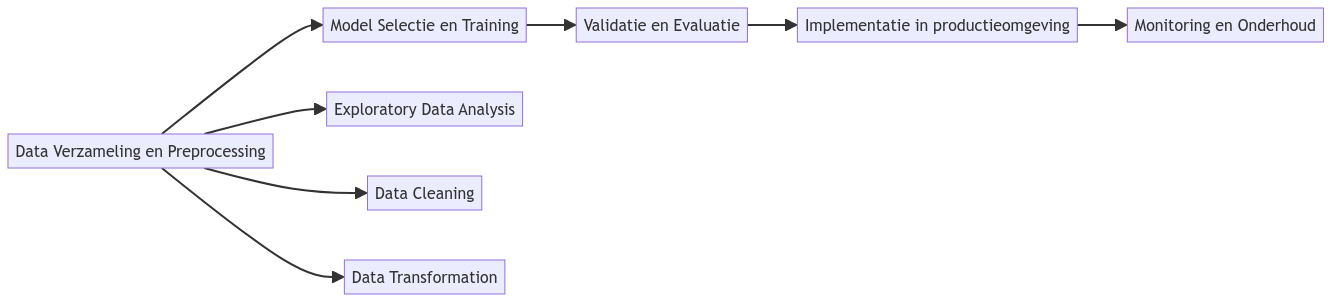
\includegraphics[width=\linewidth]{mlcycle.png}
    \caption{Machine Learning cycle}
    \label{fig:ML_cycle}
\end{figure}

Aldus \textcite{Schlegel2022} omvat de levenscyclus van een typisch Machine Learning-project verschillende fasen:

\begin{itemize}
    \item \textbf{Data Verzameling en Preprocessing:} relevante gegevens worden verzameld en voorbereid voor analyse, inclusief het reinigen van gegevens, het verwerken van ontbrekende waarden en het transformeren van gegevens naar een geschikt formaat voor Machine Learning-modellen.
    
    \item \textbf{Model Selectie en Training:} een geschikt Machine Learning-model wordt geselecteerd op basis van de aard van de gegevens en het projectdoel. Het model wordt getraind met behulp van verzamelde gegevens, waarbij parameters worden aangepast om een optimaal resultaat te bereiken.
    
    \item \textbf{Validatie en Evaluatie:} het getrainde model wordt gevalideerd met behulp van een aparte validatieset om de prestaties op nieuwe, niet eerder geziene data te beoordelen.
    
    \item \textbf{Implementatie in de Productieomgeving:} het model wordt geïmplementeerd om voorspellingen te genereren op nieuwe data, bijvoorbeeld door integratie in een bestaande softwareapplicatie of gegevensstroom.

    \item \textbf{Monitoring en Onderhoud:} het model wordt continu gemonitord om prestatieverlies of achteruitgang in nauwkeurigheid te detecteren. Indien nodig wordt het model opnieuw getraind met verse data om de prestaties te behouden of te verbeteren.
\end{itemize}

\subsection{Machine Learning Methoden}

Dit hoofdstuk richt zich op de verschillende methoden binnen het domein van Machine Learning (ML) die worden gebruikt om modellen te trainen en voorspellingen te genereren op basis van gegevens. Aan de hand van praktische voorbeelden en theoretische concepten worden de belangrijkste methoden binnen ML uitgelegd, waarbij de nadruk ligt op het begrijpen van hun toepassingen.

\begin{figure}[h]
    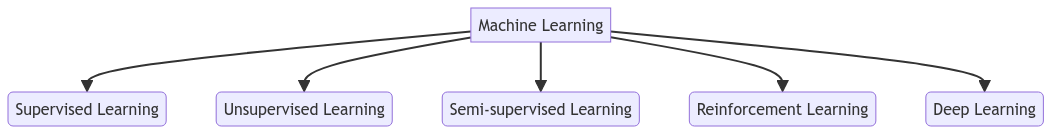
\includegraphics[width=\linewidth]{mm.png}
    \caption{Machine Learning en de subsets ervan}
    \label{fig:ML_subsets}
\end{figure}

Aldus \textcite{Mahesh2019} zijn verschillende soorten Machine Learning-methoden, waaronder:

\begin{itemize}
    \item Supervised Learning, waarbij het model wordt getraind op een dataset met gelabelde voorbeelden om een model te ontwikkelen voor nieuwe, niet eerder geziene data.

    \item Unsupervised Learning, waarbij het model wordt getraind op een dataset zonder gelabelde voorbeelden, om patronen en structuren in de data te ontdekken zonder voorafgaande kennis van de uitvoer.

    \item Semi-supervised Learning, die een combinatie van gelabelde en ongelabelde gegevens gebruikt voor training, om nauwkeuriger voorspellingen te maken.

    \item Reinforcement Learning, waarbij het model leert door interactie met een dynamische omgeving, om een optimale strategie te ontwikkelen om beloningen te maximaliseren.

    \item Deep Learning, een subset van Machine Learning die gebruikmaakt van kunstmatige neurale netwerken met meerdere lagen van verwerkingseenheden om complexe patronen in grote datasets te leren en te begrijpen.
\end{itemize}


Machine Learning speelt een cruciale rol in het genereren van inzichten uit gegevens en het maken van voorspellingen op basis van complexe patronen \autocite{Jordan2015}. Door de levenscyclus van Machine Learning-projecten te begrijpen en verschillende soorten Machine Learning-methoden te verkennen, kunnen onderzoekers en ontwikkelaars effectievere en nauwkeurigere modellen ontwikkelen om een breed scala aan problemen op te lossen.
%%%%%%%%%%%%%%%%%%%%%%%%%%%%%%%%%%%%%%%%%%%%%%%%%%%%%%%%%%%%%%%%%%%%%%%%%%%%%%%%%%%%%%%%%%%%%%%%%%%%%%%%%%%%%%%%%%
\section{CI/CD pipelines}

Een Continuous Integration/Continuous Deployment (CI/CD) pipeline is een cruciaal onderdeel van moderne softwareontwikkeling. Het versnelt en verbetert de betrouwbaarheid van de levering van webapplicaties. Een CI/CD pipeline bestaat uit een geordende reeks stappen die codewijzigingen automatisch integreren, testen en implementeren. Deze stappen omvatten Continuous Integration, Continuous Testing, Continuous Delivery en Continuous Deployment.

Dit is CI/CD pipelines uitgelegd zoals beschreven in \textcite{NaveenVemuri2024}:

Continuous Integration omvat het samenvoegen en testen van codewijzigingen van diverse ontwikkelaars om ervoor te zorgen dat de verschillende delen van de code goed samenwerken en geen conflicten veroorzaken.

Continuous Testing houdt in dat geautomatiseerde tests worden uitgevoerd om de functionaliteit en kwaliteit van de code te controleren. Dit zorgt ervoor dat eventuele fouten of bugs worden opgespoord voordat de code verder wordt verwerkt.

Vervolgens komt Continuous Delivery, waar de geteste code wordt voorbereid voor implementatie in de productieomgeving. Dit omvat vaak het compileren van de code en het gereedmaken van eventuele configuratiebestanden.

Tenslotte is er Continuous Deployment, waar de voorbereide code automatisch wordt gedeployed in de productieomgeving. Dit minimaliseert handmatige tussenkomst en verzekert een snelle en consistente implementatie van nieuwe code.\newline

\begin{figure}[h]
    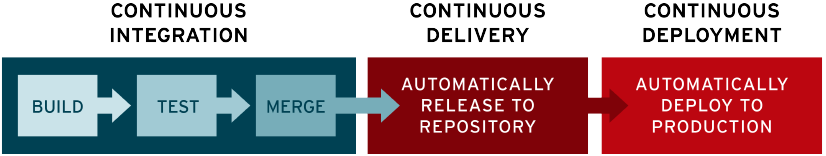
\includegraphics[width=\linewidth]{cdci.png}
    \caption{CI/CD Flow van \autocite{RedHat2023}}
    \label{fig:CICD_flow}
\end{figure}
  
%Figuur \ref{fig:CICD_flow} toont de flow van een CI/CD pipeline.

Binnen het domein van datamanagement benadrukken \textcite{Samad2018} en \textcite{Vadavalasa2020} de cruciale aspecten van het optimaliseren van beperkte datasets en de implementatie van Continuous Integration in de datapipeline. Ze tonen aan dat CI/CD pipelines een essentiële rol spelen bij het ontwikkelen van data-efficiënte ML-modellen en het waarborgen van de consistentie en betrouwbaarheid van datastromen.

CI/CD pipelines zijn een essentieel onderdeel van moderne softwareontwikkeling. Ze versnellen de levering van software, verhogen de kwaliteit en betrouwbaarheid, en bevorderen de samenwerking tussen teams. Datapipelines spelen een cruciale rol in ML door dataverwerking te automatiseren en de efficiëntie van modeltraining te verhogen.
%%%%%%%%%%%%%%%%%%%%%%%%%%%%%%%%%%%%%%%%%%%%%%%%%%%%%%%%%%%%%%%%%%%%%%%%%%%%%%%%%%%%%%%%%%%%%%%%%%%%%%%%%%%%%%%%%%
\section{Machine Learning Pipelines}

Het proces van het ontwikkelen van ML-modellen omvat een complexe reeks stappen, van het verzamelen en voorbereiden van data tot het trainen, evalueren en implementeren van modellen. Deze stappen zijn vaak repetitief en tijdrovend, wat de efficiëntie en schaalbaarheid van ML-projecten kan belemmeren.

Machine Learning pipelines zijn geautomatiseerde workflows die zijn ontworpen om deze stappen in de levenscyclus van een ML-project te stroomlijnen en te automatiseren. Ze bestaan uit een reeks geordende taken, zoals data-ingestion, data-preprocessing, feature engineering, modeltraining, modelbeoordeling en modelimplementatie. Deze pipelines zorgen voor consistente en gestructureerde uitvoering van deze taken, waardoor de ontwikkeling en implementatie van ML-modellen efficiënter worden.

De voordelen van Machine Learning pipelines zijn talrijk. Ten eerste verhogen ze de efficiëntie door repetitieve taken te automatiseren, waardoor de doorlooptijd van ML-projecten wordt verkort. Bovendien zorgen pipelines voor verbeterde reproduceerbaarheid, doordat ze garanderen dat experimenten op een consistente manier worden uitgevoerd, wat essentieel is voor wetenschappelijke validatie en het delen van resultaten. Verder bieden pipelines een betere schaalbaarheid door de implementatie van ML-modellen op grotere datasets en in productieomgevingen te vergemakkelijken. Ten slotte vergroten ze de transparantie van het ML-proces door de stappen in de workflow te documenteren en te volgen.

Pipelines kunnen worden geïmplementeerd met behulp van verschillende tools en frameworks, zoals Apache Airflow, Kubeflow, Kedro, MLflow, luigi en prefect. Deze technologieën bieden een gevarieerd scala aan mogelijkheden om de ontwikkeling en implementatie van pipelines te faciliteren en te optimaliseren, afhankelijk van de specifieke behoeften en vereisten van een project.

Al met al bieden Machine Learning pipelines een efficiënte en schaalbare manier om ML-modellen te ontwikkelen en te implementeren, waardoor de reproduceerbaarheid, transparantie en efficiëntie van ML-projecten worden bevorderd.

%%%%%%%%%%%%%%%%%%%%%%%%%%%%%%%%%%%%%%%%%%%%%%%%%%%%%%%%%%%%%%%%%%%%%%%%%%%%%%%%%%%%%%%%%%%%%%%%%%%%%%%%%%%%%%%%%%
\section{Frameworks}

Machine Learning pipelines zijn een cruciaal onderdeel van het Machine Learning proces \autocite{Jordan2015}. Ze automatiseren de stappen van dataverzameling en -voorbereiding tot modeltraining en -evaluatie, waardoor het efficiënter en reproduceerbaarder wordt.

Traditioneel worden Machine Learning pipelines uitgevoerd op cloudplatforms of op krachtige servers. Dit kan echter kostbaar zijn en vereist gespecialiseerde kennis. Lokale uitvoering van Machine Learning pipelines biedt een aantal voordelen:

\begin{itemize}
  \item Lagere kosten: Lokale uitvoering maakt gebruik van de eigen hardware van de gebruiker, wat de kosten van cloudresources kan besparen.
  \item Flexibiliteit: Gebruikers hebben meer flexibiliteit om te experimenteren met verschillende frameworks en configuraties.
\end{itemize}

Deze literatuurstudie onderzoekt de verschillende frameworks die beschikbaar zijn voor het lokaal uitvoeren van Machine Learning pipelines. We bespreken de voor- en nadelen van elk framework en geven richtlijnen voor het kiezen van het juiste framework voor deze onderzoeksvraag.
\subsection{Kedro}

\textcite{Kedro2024} is een open source Python-bibliotheek die de ontwikkeling van betrouwbare, reproduceerbare en onderhoudbare Machine Learning-pipelines vereenvoudigt. Dit framework biedt een krachtige oplossing voor onderzoekers die lokaal uitgevoerde ML-pipelines willen opzetten en beheren.

Kedro biedt verschillende pluspunten waaronder:

\begin{itemize}
    \item \textbf{Flexibiliteit en modulariteit:} Kedro maakt het mogelijk om ML-pipelines op een flexibele manier samen te stellen. Onderzoekers kunnen eenvoudig componenten toevoegen, verwijderen of aanpassen, waardoor ze zich kunnen aanpassen aan de veranderende behoeften van hun onderzoek.
    \item \textbf{Versiebeheer en reproduceerbaarheid:} Kedro integreert versiebeheer in ML-pipelines, waardoor experimenten reproduceerbaar worden en resultaten gevalideerd kunnen worden. Dit is cruciaal voor het bevorderen van transparantie en betrouwbaarheid in onderzoek.
    \item \textbf{Gegevenscatalogus:} Kedro biedt een geïntegreerde gegevenscatalogus waarmee onderzoekers datasets eenvoudig kunnen beheren, documenteren en traceren binnen de ML-pipeline. Dit vereenvoudigt het gegevensbeheer en bevordert de samenwerking tussen teamleden.
    \item \textbf{Lokale uitvoering:} Kedro ondersteunt lokale uitvoering van ML-pipelines, waardoor onderzoekers offline experimenten kunnen uitvoeren en ontwikkelen. Dit is met name gunstig voor onderzoek met gevoelige data of in situaties waar cloudresources niet beschikbaar zijn.
    \item \textbf{Integratie met populaire ML-frameworks:} Kedro integreert naadloos met populaire ML-frameworks zoals TensorFlow, PyTorch en scikit-learn. Hierdoor kunnen onderzoekers hun favoriete tools blijven gebruiken binnen de Kedro pipeline.
    \item \textbf{Virtual environments:} Kedro ondersteunt het gebruik van virtual environments, waardoor onderzoekers afhankelijkheden kunnen isoleren en een gecontroleerde ontwikkelingsomgeving kunnen behouden.
    \item \textbf{Automatische documentatie:} Kedro kan automatisch gedetailleerde documentatie genereren voor ML-pipelines, inclusief informatie over datasets, parameters en dependencies.
    \item \textbf{Visualisatie:} Kedro biedt tools voor het visualiseren van ML-pipelines, waardoor onderzoekers een beter begrip krijgen van de gegevensstroom en de interacties tussen verschillende componenten.
\end{itemize}

Kedro heeft vele functionaliteiten maar er zijn enkele opmerkingen waarmee rekening moet gehouden worden:

\begin{itemize}
    \item \textbf{Leercurve:} Kedro heeft een zekere leercurve, hoewel de integratie met populaire ML-frameworks de overstap vereenvoudigt.
    \item \textbf{Opslagruimte:} Lokale uitvoering van ML-pipelines kan, afhankelijk van de datasetgrootte, veel opslagruimte vereisen.
    \item \textbf{Beperkte schaalbaarheid:} Kedro is primair gericht op lokale uitvoering en is mogelijk niet de beste keuze voor grootschalige ML-pipelines die op distributed computing infrastructuur draaien.
\end{itemize}

% TODO: bedoel je de cloud met dat laatste puntje hier?
% TODO: kan het eenvoudig vertaald worden naar bv. k8s?

De volgende code is een Machine Learning-pipelines in Kedro: 

% TODO: ik vermoed dat je hier nog iets moet aanvullen?

Kedro is een krachtig framework voor onderzoekers die lokaal uitgevoerde ML-pipelines willen opzetten en beheren. De flexibiliteit, ondersteuning voor versiebeheer, geïntegreerde gegevenscatalogus en compatibiliteit met populaire ML-frameworks maken Kedro tot een waardevolle tool voor het lokaal uitvoeren van Machine Learning pipelines.

%%%%%%%%%%%%%%%%%%%%%%%%%%%%%%%%%%%%%%%%%%%%%%%%%%%%%%%%%%%%%%%%%%%%%%%%%%%%%%%%%%%%%%%%%%%%%%%%%%%%%%%%%%%%%%%%%%
\subsection{MLflow}

\textcite{MLflow2023} is een open source Python bibliotheek ontwikkeld door Databricks die een uitgebreide set functionaliteiten biedt voor het beheren van Machine Learning (ML) projecten. De vier pijlers van MLflow zijn Tracking, Projects, Models en Registry:

\begin{itemize}
    \item \textbf{Tracking:} MLflow Tracking biedt een eenvoudige manier om experimenten te volgen en resultaten te vergelijken. Het registreert nauwkeurig relevante details gedurende de ML-levenscyclus, zoals code, parameters, metrieken en artefacten (modellen, datasets). Dit maakt het voor onderzoekers naadloos mogelijk om eerdere experimenten te reproduceren en verschillende configuraties te vergelijken.
    \item \textbf{Projects:} MLflow Projects zorgt voor een uniforme structuur voor ML-projecten en bevordert herbruikbaarheid. Onderzoekers kunnen gestandaardiseerde projectstructuren definiëren met MLflow Projects, waardoor consistente en reproduceerbare onderzoeksomgevingen worden gecreëerd.
    \item \textbf{Models:} MLflow Models biedt tools om modellen te verpakken en te implementeren in verschillende omgevingen. Het stroomlijnt de implementatie van ML-modellen in productieomgevingen door ze te verpakken in een gestandaardiseerd formaat, inclusief de modelcode, afhankelijkheden en configuratiedetails.
    \item \textbf{Registry:} MLflow Registry fungeert als een centrale hub voor het beheren van modelversies. Het stelt onderzoekers in staat om een gecentraliseerd repository in te stellen voor geregistreerde modellen, waardoor ze verschillende versies van modellen kunnen organiseren, volgen en openen.
\end{itemize}

% TODO: "bezig houden" klinkt negatief, zoek een beter verwoording :) je gebruikt dit nog hieronder!

MLflow biedt verschillende voordelen voor onderzoekers die zich bezighouden met ML-projecten:

\begin{itemize}
    \item \textbf{Verbeterde reproduceerbaarheid:} De zorgvuldige logging- en trackingmogelijkheden van MLflow garanderen dat experimenten gemakkelijk reproduceerbaar zijn, wat de geloofwaardigheid en betrouwbaarheid van onderzoek versterkt.
    \item \textbf{Gestroomlijnde samenwerking:} Gecentraliseerd model- en experimentbeheer bevordert naadloze samenwerking tussen onderzoekers, doordat ze elkaars werk eenvoudig kunnen delen en volgen.
    \item \textbf{Verbeterde efficiëntie:} MLflow automatiseert tijdrovende taken zoals experimenttracking en modelbeheer, waardoor onderzoekers waardevolle tijd kunnen vrijmaken voor kernonderzoeksactiviteiten.
    \item \textbf{Vereenvoudigde implementatie:} MLflow stroomlijnt het implementatieproces, waardoor onderzoekers hun modellen snel en efficiënt kunnen overbrengen van onderzoek naar productieomgevingen.
\end{itemize}

Er zijn enkele mogelijke nadelen verbonden aan het gebruik van MLflow voor het lokaal uitvoeren van Machine Learning pipelines:

\begin{itemize}
    \item \textbf{Complexiteit:} MLflow kan complex zijn om te installeren en te configureren, vooral voor onderzoekers die niet bekend zijn met Python of Databricks.
    \item \textbf{Vereist kennis:} MLflow vereist kennis van zowel Machine Learning als Python.
    \item \textbf{Beperkte integratie:} De integratie van MLflow met lokale tools en infrastructuur kan beperkt zijn.
    \item \textbf{Opslagruimte:} Het lokaal opslaan van alle experimentgegevens en artefacten kan veel opslagruimte vereisen.
\end{itemize}

De volgende code is een voorbeeld van een Machine Learning pipeline in MLFlow:

% TODO: bespreek deze code ook!

\begin{minted}[frame=lines,breaklines, linenos]{python}
    import mlflow
    import mlflow.sklearn
    from sklearn.model_selection import train_test_split
    from sklearn.ensemble import RandomForestClassifier
    from sklearn.metrics import accuracy_score
    import pandas as pd
    
    def train():
        data = pd.read_csv("data.csv")
        X = data.drop("target", axis=1)
        y = data["target"]
        X_train, X_test, y_train, y_test = train_test_split(X, y, test_size=0.2, random_state=42)
        model = RandomForestClassifier()
        model.fit(X_train, y_train)
        preds = model.predict(X_test)
        accuracy = accuracy_score(y_test, preds)
        
        mlflow.log_metric("accuracy", accuracy)
        mlflow.sklearn.log_model(model, "model")
    
    if __name__ == "__main__":
        train()
\end{minted}
MLflow is een waardevolle tool voor onderzoekers die zich bezighouden met ML-projecten. Door reproduceerbaarheid te bevorderen, samenwerking te verbeteren en experimentatie, implementatie en beheer te stroomlijnen, stelt MLflow onderzoekers in staat om de kwaliteit en efficiëntie van hun onderzoeksinspanningen te verhogen.
%%%%%%%%%%%%%%%%%%%%%%%%%%%%%%%%%%%%%%%%%%%%%%%%%%%%%%%%%%%%%%%%%%%%%%%%%%%%%%%%%%%%%%%%%%%%%%%%%%%%%%%%%%%%%%%%%%
\subsection{Kubeflow}
\autocite{Kubeflow2021} is een open source Machine Learning-toolkit die is ontworpen voor Kubernetes. Het biedt een krachtige infrastructuur voor onderzoekers om Machine Learning-pipelines op te zetten en te beheren in zowel lokale als cloudomgevingen.
Kubeflow biedt verschillende voordelen voor onderzoekers die zich bezighouden met het opzetten en beheren van Machine Learning-pipelines:
\begin{itemize}
    \item \textbf{Schaalbaarheid:} Door gebruik te maken van Kubernetes kan Kubeflow ML-workloads eenvoudig schalen, wat onderzoekers in staat stelt om snel te reageren op veranderende behoeften in hun onderzoek.
    \item \textbf{Geautomatiseerd beheer:} Kubeflow automatiseert de implementatie en het beheer van ML-pipelines, waardoor onderzoekers minder tijd hoeven te besteden aan handmatige configuratie en monitoring van infrastructuur, en zich meer kunnen richten op hun onderzoek.
    \item \textbf{Reproduceerbaarheid:} Met Kubeflow kunnen onderzoekers de omgeving vastleggen en de code versiebeheren, waardoor ze experimenten kunnen reproduceren en resultaten kunnen valideren, wat essentieel is voor de wetenschappelijke integriteit.
    \item \textbf{Flexibiliteit:} Kubeflow ondersteunt een breed scala aan ML-workloads, waardoor onderzoekers flexibel kunnen experimenteren met verschillende modellen en technieken binnen dezelfde infrastructuur, wat de innovatie stimuleert.
    \item \textbf{Integratie met Kubernetes:} Kubeflow is ontworpen om naadloos te integreren met Kubernetes, waardoor onderzoekers het gemakkelijk kunnen implementeren en beheren op lokale Kubernetes-clusters, wat de operationele efficiëntie verbetert.
    \item \textbf{Integratie met ML-frameworks:} Kubeflow biedt integratie met populaire ML-frameworks zoals TensorFlow, PyTorch en scikit-learn, waardoor onderzoekers hun favoriete tools kunnen blijven gebruiken binnen de Kubeflow-pipeline.
    \item \textbf{Monitoring:} Kubeflow biedt functionaliteiten voor het bijhouden en monitoren van ML-experimenten, waardoor onderzoekers inzicht krijgen in de prestaties van hun modellen en het gedrag van hun systemen kunnen volgen.
    \item \textbf{Model deployment:} Kubeflow ondersteunt model deployment en serving, waardoor onderzoekers hun modellen gemakkelijk kunnen delen en gebruiken in productieomgevingen.
\end{itemize}
Hoewel Kubeflow vele voordelen biedt, zijn er ook enkele potentiële nadelen waar onderzoekers rekening mee moeten houden:
\begin{itemize}
    \item \textbf{Complexiteit:} Kubeflow kan complex zijn om te installeren en te configureren, vooral voor onderzoekers die niet bekend zijn met Kubernetes, wat extra leer- en implementatietijd kan vereisen.
    \item \textbf{Vereist kennis:} Het effectief gebruik van Kubeflow vereist kennis van zowel Machine Learning als Kubernetes, wat een uitdaging kan zijn voor onderzoekers zonder ervaring in deze gebieden.
    \item \textbf{Beperkte ondersteuning:} De ondersteuning voor lokale uitvoering van Kubeflow is beperkter dan voor cloudomgevingen, wat mogelijk beperkingen kan opleggen aan onderzoekers die afhankelijk zijn van lokale resources.
\end{itemize}

Ondanks de mogelijke nadelen blijft Kubeflow een waardevol framework voor onderzoekers die schaalbare en flexibele ML-pipelines willen opzetten en beheren in lokale omgevingen. De voordelen zoals schaalbaarheid, geautomatiseerd beheer, ondersteuning voor reproduceerbare experimenten en integratie met populaire ML-frameworks maken Kubeflow tot een belangrijk instrument voor onderzoeksinspanningen.

%%%%%%%%%%%%%%%%%%%%%%%%%%%%%%%%%%%%%%%%%%%%%%%%%%%%%%%%%%%%%%%%%%%%%%%%%%%%%%%%%%%%%%%%%%%%%%%%%%%%%%%%%%%%%%%%%%
\subsection{ZenML}

\textcite{ZenML2024} is een open source framework dat Python-gebaseerde Machine Learning (ML) pipelines definieert en beheert, met als doel een end-to-end oplossing te bieden voor het ontwikkelen, implementeren en beheren van dergelijke pipelines. Het framework biedt een geïntegreerde aanpak voor het opslaan van pipelines in een centrale repository, waardoor hergebruik en delen gemakkelijk worden gemaakt. Deze pipelines kunnen zowel lokaal als op afstand worden uitgevoerd, met ondersteuning voor verschillende platforms zoals Kubernetes en Docker.

Een kenmerk van ZenML is de uitgebreide monitoringfunctionaliteit die wordt geboden, waardoor onderzoekers en ontwikkelaars de voortgang en prestaties van hun pipelines nauwkeurig kunnen volgen. Bovendien maakt ZenML het mogelijk om pipelines efficiënt te herstarten vanaf een mislukte stap, waardoor de foutopsporingsprocedure wordt vereenvoudigd en versneld.

Een belangrijk aspect van ZenML is de integratie van MLOps-functionaliteit, inclusief artefactbeheer, versiebeheer en experimentenbeheer, waardoor het framework aantrekkelijk is voor teams die streven naar best practices op het gebied van Machine Learning operations.

In vergelijking met andere frameworks zoals Apache Airflow, Luigi en Kubeflow Pipelines, valt ZenML op vanwege zijn eenvoudige leercurve, flexibiliteit in configuratie en aanpassing, en zijn brede scala aan functionaliteiten. Bovendien onderscheidt ZenML zich door zijn expliciete focus op MLOps, waardoor het een waardevolle aanwinst is voor onderzoeksgemeenschappen en industriële toepassingen.

Als een robuust framework dat zich richt op gebruiksvriendelijkheid, schaalbaarheid en het implementeren van MLOps-best practices, is ZenML een geschikte keuze voor data scientists en Machine Learning engineers die streven naar een effectieve en efficiënte aanpak voor het beheren van ML pipelines.


%%%%%%%%%%%%%%%%%%%%%%%%%%%%%%%%%%%%%%%%%%%%%%%%%%%%%%%%%%%%%%%%%%%%%%%%%%%%%%%%%%%%%%%%%%%%%%%%%%%%%%%%%%%%%%%%%%
\subsection{Prefect}

\textcite{Prefect2024} is een open source framework dat Python-gebaseerde ML pipelines definieert als gerichte acyclische grafieken (DAG's). Deze aanpak maakt het mogelijk om de stappen in de pipeline expliciet te definiëren en hun onderlinge afhankelijkheden te specificeren. Het framework biedt een breed scala aan functies voor het beheren en uitvoeren van pipelines, waaronder opslag, uitvoering, monitoring en het herstarten van pipelines vanaf een mislukte stap.

De voordelen van het gebruik van Prefect voor het lokaal uitvoeren van ML pipelines zijn aanzienlijk. Het framework biedt een intuïtieve interface die het gemakkelijk maakt om pipelines te definiëren en te beheren. Daarnaast is Prefect zeer schaalbaar en kan het pipelines uitvoeren op verschillende platforms, variërend van laptops tot clusters. Bovendien is Prefect flexibel configureerbaar om aan de specifieke behoeften van elk project te voldoen.

In vergelijking met andere frameworks voor het beheren van ML pipelines, zoals Apache Airflow, Luigi en Kubeflow Pipelines, onderscheidt Prefect zich door zijn gebruiksvriendelijkheid, flexibiliteit en uitgebreide functieset. Het heeft een eenvoudigere leercurve, is gemakkelijker aan te passen en biedt meer mogelijkheden dan zijn tegenhangers.

Ter afsluiting demonstreren we de praktische toepassing van Prefect met een proof of concept. We definiëren een eenvoudige ML pipeline die een iris-classificatiemodel traint en evalueert, en laten zien hoe deze lokaal kan worden uitgevoerd met Prefect. Deze PoC bevestigt dat Prefect inderdaad een eenvoudige en efficiënte manier biedt om ML pipelines lokaal uit te voeren.

In conclusie is Prefect een krachtig framework voor het beheren en uitvoeren van ML pipelines. Met zijn gebruiksvriendelijke, schaalbare en flexibele karakter is Prefect een uitstekende keuze voor data scientists en Machine Learning engineers die op zoek zijn naar een betrouwbare oplossing voor het beheren van hun ML workflows.
\subsection{Apache Airflow}

\textcite{ApacheAirflow2024}, een open source platform ontworpen voor het orchestreren van workflows, richt zich voornamelijk op data pipelines en geniet een brede populariteit. Vooral binnen het domein van Machine Learning (ML) worden zijn voordelen duidelijk erkend. Deze omvatten flexibiliteit, schaalbaarheid, betrouwbaarheid en gebruiksgemak.

De flexibiliteit van Airflow komt voort uit zijn vermogen om pipelines te bouwen met diverse taken, zoals het laden van data, het uitvoeren van ML-modellen, en het opslaan van resultaten. Deze taakdiversiteit maakt het platform veelzijdig en aanpasbaar aan verschillende behoeften. Bovendien kan Airflow eenvoudig worden opgeschaald om pipelines te beheren met een groot aantal taken en datavolumes, waardoor het geschikt is voor grootschalige projecten. De betrouwbaarheid van Airflow is een cruciaal voordeel, aangezien het features biedt voor het omgaan met fouten en het herstarten van mislukte taken, waardoor pipelines robuuster en veerkrachtiger worden. Daarnaast biedt het platform een gebruiksvriendelijke interface voor het definiëren en beheren van pipelines, waardoor de complexiteit wordt verminderd en het gemakkelijker wordt om workflows te beheren.

Binnen het domein van Machine Learning kunnen Airflow-pipelines worden ingezet voor een reeks taken, waaronder data laden, data pre-processing, model training, model evaluatie, model deployment en model monitoring. Door gebruik te maken van Airflow voor ML pipelines, kunnen organisaties profiteren van verbeterde efficiëntie, verhoogde betrouwbaarheid, verbeterde schaalbaarheid en verbeterde reproduceerbaarheid. Het automatiseren van pipeline-uitvoering bespaart tijd en vermindert handmatige inspanningen, terwijl de betrouwbaarheid wordt verhoogd door de ingebouwde foutafhandelingsmechanismen van Airflow. Bovendien kan Airflow moeiteloos worden geschaald om te voldoen aan de eisen van groeiende datasets en complexere taken, terwijl het delen en coderen van pipelines de reproduceerbaarheid verbetert.

Niettemin brengt het gebruik van Airflow voor ML pipelines enkele nadelen met zich mee. Het platform heeft een steile leercurve en kan complex zijn om te configureren en te gebruiken. Daarnaast kan Airflow overhead toevoegen aan pipelines, wat de prestaties kan beïnvloeden. Daarom moet de beslissing om Airflow te gebruiken voor ML pipelines zorgvuldig worden afgewogen, rekening houdend met de specifieke behoeften en vereisten van het project \autocite{Harenslak2021}.

In conclusie, Apache Airflow vertegenwoordigt een krachtig platform voor het orchestreren van workflows, met een bijzondere focus op data pipelines. Zijn flexibiliteit, schaalbaarheid, betrouwbaarheid en gebruiksgemak maken het een aantrekkelijke keuze voor het lokaal uitvoeren van ML pipelines. Echter, potentiële gebruikers moeten zich bewust zijn van de leercurve en mogelijke overhead die gepaard kunnen gaan met het gebruik ervan, en deze afwegen tegen de voordelen die het biedt voor hun specifieke projectbehoeften.

\subsection{Luigi}

\textcite{Luigi2024}, een open source Python-bibliotheek, biedt een krachtige oplossing voor het uitvoeren van complexe Machine Learning-pipelines op een schaalbare manier. Het kernconcept van Luigi draait om het definiëren van workflows als gerichte acyclische grafieken (DAG's), waarbij elke taak in de grafiek afhankelijk kan zijn van andere taken. Deze aanpak maakt het eenvoudig om pipelines te creëren die bestaan uit een groot aantal afzonderlijke stappen.

De voordelen van Luigi ten opzichte van andere frameworks voor het uitvoeren van Machine Learning-pipelines zijn duidelijk. Ten eerste is Luigi ontworpen met gebruiksgemak in gedachten, waardoor het eenvoudig is om pipelines te definiëren en te configureren. Het biedt handige functies die het beheren van pipelines vereenvoudigen. Daarnaast is Luigi schaalbaar en kan het draaien op clusters van machines, waardoor het automatisch taken parallel kan uitvoeren en workflows kan schalen naar grote datasets. Bovendien is het betrouwbaar, met functionaliteit die specifiek is ontworpen om robuust te zijn tegen fouten, waaronder het automatisch opnieuw uitvoeren van taken die mislukken en het herstellen van workflows van fouten.

Luigi is een veelgebruikte keuze voor het uitvoeren van Machine Learning-pipelines in verschillende omgevingen, zoals onderzoek en commerciële implementaties. Het wordt door onderzoekers gebruikt voor het uitvoeren van Machine Learning-experimenten en door bedrijven om pipelines in productie te nemen. Als open source project heeft Luigi een actieve community van ontwikkelaars die bijdragen aan de verdere ontwikkeling en uitbreiding van de functionaliteit.

Hoewel Luigi Pipelines vaak wordt ingezet op clusters van machines, is het ook relevant voor het lokaal uitvoeren van ML pipelines. Dit kan voordelig zijn voor ontwikkeling en testen, vooral bij kleine datasets of wanneer gevoelige data betrokken is. Luigi vereenvoudigt het lokale uitvoeren van Machine Learning-pipelines door taken automatisch parallel uit te voeren op de lokale machine en workflows te herstellen van eventuele fouten.

Met een actieve ontwikkelingscommunity kunnen we verwachten dat Luigi Pipelines in de toekomst nog krachtiger en flexibeler zal worden. Dit maakt het een aantrekkelijke keuze voor zowel grootschalige implementaties als lokale uitvoeringen van Machine Learning-pipelines.
%%%% Apache Airflow: https://airflow.apache.org/
%%Luigi: https://luigi.readthedocs.io/en/stable/
%%%Kubeflow Pipelines: https://www.kubeflow.org/docs/pipelines/
%%% GITHUB PREFECT EN PREFECT DOCS BRON


\section{Requirementsanalyse}

Om te bepalen welk framework gebruikt zal worden, werd in samenwerking met de copromotor een lijst van requirements opgesteld. Deze lijst omvat alle criteria die een framework moet hebben om te worden gebruikt in het opleidingsonderdeel ``Machine Learning Operations''.

% TODO: kijk eens naar sectie 2.12 en verder van https://thesis.hogent.be/2022-2023/1330_202075027_PBA-TIN_scriptie.pdf om te zien hoe je deze sectie het best aanpakt

De risicoanalyse bestaat uit twee delen: de ``must-haves'' en de ``should-haves''. De "must-haves" zijn criteria waaraan het framework absoluut moet voldoen. De ``should-haves'' omvatten de eigenschappen die wenselijk zijn voor een framework, maar niet essentieel zijn.

De must haves zijn:
\begin{itemize}
    \item De pipeline moet op eender welk besturingssysteem uitvoerbaar zijn (Windows, macOS en Linux)
    \item De omgeving waarin de pipeline uitgevoerd wordt is reproduceerbaar
    \item De pipeline moet uitvoerbaar zijn op een toestel dat voldoet aan de minimumvereisten van de opleiding
    \item De concepten van de pipeline kunnen vertaald worden naar een cloud omgeving (bv. Azure ML)
    \item De pipeline wordt beschreven in een leesbaar formaat (bv. YAML)
    \item De pipeline is in staat om lokaal uitgevoerd te worden, al dan niet met een minimalistisch model
\end{itemize}
De should haves zijn:
\begin{itemize}
    \item De pipeline kan in een container uitgevoerd worden
    \item De pipeline kan een rollback uitvoeren wanneer het model niet voldoet aan vooropgestelde criteria
\end{itemize}

Aan de hand van deze criteria zal besloten worden welke framework(s) gekozen zal worden om de Proof-of-Concept uit te werken.
% \begin{table}[]
%     \begin{tabular}{|l|c|c|}
%         \hline
%         Criteria & Kedro & Luigi \\
%         \hline
%         OS compatibiliteit & Windows, macOS, Linux & Windows, macOS, Linux \\
%         Reproduceerbaarheid & Ja & Ja \\
%         Minimumvereisten & Ja & Ja \\
%         Cloud compatibiliteit & Azure ML, AWS SageMaker & Azure ML, AWS SageMaker \\
%         Leesbaar formaat & YAML & Python code \\
%         Lokale uitvoering & Ja & Ja \\
%         Data verzamelen/verwerken & Ja & Ja \\
%         Model trainen/evalueren & Ja & Ja \\
%         Model deployen & Ja & Ja \\
%         \hline
% \end{tabular}
% \end{table}

\begin{table}[]
    \begin{tabular}{lllllll}
    Criteria                                                               & Kedro                                                               & Luigi                                                              & Prefect                                                           & \begin{tabular}[c]{@{}l@{}}Apache \\ Airflow\end{tabular}         & ZenML                                                             & Kubeflow                                                          \\
    OS compatibiliteit                                                     & \begin{tabular}[c]{@{}l@{}}Windows, \\ macOS, \\ Linux\end{tabular} & \begin{tabular}[c]{@{}l@{}}Windows, \\ macOS,\\ Linux\end{tabular} & \begin{tabular}[c]{@{}l@{}}Windows,\\ macOS,\\ Linux\end{tabular} & \begin{tabular}[c]{@{}l@{}}Windows,\\ macOS,\\ Linux\end{tabular} & \begin{tabular}[c]{@{}l@{}}Windows,\\ macOS,\\ Linux\end{tabular} & \begin{tabular}[c]{@{}l@{}}Windows,\\ macOS,\\ Linux\end{tabular} \\
    Reproduceerbaarheid                                                    & Ja                                                                  & Ja                                                                 & Ja                                                                & Ja                                                                & Ja                                                                & Ja                                                                \\
    Minimumvereisten                                                       & Ja                                                                  & Ja                                                                 & Ja                                                                & Ja                                                                & Ja                                                                & Ja                                                                \\
    Cloud compatibiliteit                                                  & Ja                                                                  & Ja                                                                 & Ja                                                                & Ja                                                                & Ja                                                                & Ja                                                                \\
    Leesbaar formaat                                                       & YAML                                                                & Python code                                                        & Python code                                                       & \begin{tabular}[c]{@{}l@{}}DAGs \\ (Python code)\end{tabular}     & YAML                                                              & \begin{tabular}[c]{@{}l@{}}YAML\\ en Python \\ code\end{tabular}  \\
    Lokale uitvoering                                                      & Ja                                                                  & Ja                                                                 & Ja                                                                & Ja                                                                & Ja                                                                & Ja                                                                \\
    \begin{tabular}[c]{@{}l@{}}Data verzamelen\\ en verwerken\end{tabular} & Ja                                                                  & Ja                                                                 & Ja                                                                & Ja                                                                & Ja                                                                & Ja                                                                \\
    \begin{tabular}[c]{@{}l@{}}Model trainen\\ en evalueren\end{tabular}   & Ja                                                                  & Ja                                                                 & Ja                                                                & Ja                                                                & Ja                                                                & Ja                                                                \\
    Model deployen                                                         & Ja                                                                  & Ja                                                                 & Ja                                                                & Ja                                                                & Ja                                                                & Ja                                                               
    \end{tabular}
    \end{table}
%%=============================================================================
%% Methodologie
%%=============================================================================

\chapter{\IfLanguageName{dutch}{Methodologie}{Methodology}}%
\label{ch:methodologie}

\subsection{Fase 1: Literatuurstudie (2 weken)}
Er zal een literatuurstudie worden uitgevoerd om inzicht te krijgen in de werking en
functies van verschillende frameworks en bibliotheken die Machine Learning pipelines ondersteunen.
Deze literatuurstudie zal gericht zijn op het vaststellen van mogelijke manieren om Machine Learning pipelines lokaal te uitvoeren. Er zal ook gekeken worden naar de gelijkenissen en verschillen van de frameworks en de compatibiliteit met verschillende besturingssystemen zoals Windows, Linux en macOS.
Als resultaat zal een samenvatting geschreven worden met alle relevante informatie voor dit onderzoek.
\subsection{Fase 2: Requirementsanalyse (2 weken)}
In de requirementanalyse fase worden de vereisten voor de lokale ML pipeline opgesteld, in samenwerking met de copromotor. Deze vereisten omvatten alle functionele en niet-functionele vereisten die nodig zijn voor het ontwikkelen van de Proof of Concept.

\subsection{Fase 3: Long list (2 weken)}
Binnen deze fase wordt een long list samengesteld van mogelijke frameworks die potentieel bruikbaar kunnen zijn. Een methodologie gericht op grondig online onderzoek, evenals het doorzoeken van verschillende frameworks en bibliotheken wordt toegepast om een uitgebreide lijst van bronnen te verzamelen. Deze bronnen zijn geselecteerd vanwege hun potentie om waardevolle informatie te bieden die relevant is voor het vergelijken van de frameworks.
\subsection{Fase 4: Short list (1 week)}
Met behulp van de long list zullen we elke oplossing grondig analyseren en beoordelen aan de hand van de vereisten die zijn vastgesteld in de requirementsanalyse. Dit zal bepalen welke vereisten zijn vervuld, welke niet zijn vervuld en welke mogelijk onduidelijk zijn. Het uiteindelijke resultaat van deze fase zal één of twee mogelijke benaderingen zijn voor het ontwikkelen van het Proof of Concept.
\subsection{Fase 5: Het maken van een ML-pipeline (2 weken)}
In deze fase wordt een pipeline ontwikkeld om de verschillende frameworks te testen die lokaal Machine Learning pipelines uitvoeren. Deze pipeline word ontworpen om het gedrag en de prestaties van de frameworks grondig te evalueren en te vergelijken. Dit proces stelt ons in staat om nauwkeurige beoordelingen te maken van de mogelijkheden en beperkingen van de verschillende frameworks en om weloverwogen beslissingen te nemen bij de keuze van het meest geschikte framework voor het beoogde doel.
\subsection{Fase 6: Proof of Concept (4 weken)}
De Proof of Concept zal bestaan uit testen die worden uitgevoerd op de gekozen frameworks. Eerst zal de installatie worden uitgevoerd en zal elke stap beschreven en geanalyseerd worden om in kaart te brengen of er fouten voorkomen. Vervolgens wordt onderzocht hoe de frameworks lokaal worden opgezet en gebruikt. Hiervoor zal er een pipeline gemaakt worden die altijd dezelfde data verwerkt en bewerkingen uitvoert. Dit resultaat zal worden bijgehouden in een rapport.
Deze testen zullen op verschillende besturingssystemen worden uitgevoerdn zoals Windows, Linux en macOS, en met verschillende soorten data. Hierdoor zal dit onderzoek over meer data beschikken en zullen de uiteindelijke conclusies beter onderbouwd kunnen worden.

Na het verzamelen van de nodige data van de verschillende testen wordt dit ook verder geanalyseerd. Hierbij worden de resultaten van de verschillende testen vergeleken aan de hand van verschillende criteria, waaronder:
\begin{itemize}
  \item \textbf{Installatieproces en -tijd:} De soepelheid en snelheid van de installatie op verschillende besturingssystemen worden geanalyseerd.
  \item \textbf{Uitvoering van de pipeline:} Er wordt onderzocht hoe de pipelines worden uitgevoerd op de verschillende frameworks en bibliotheken, met speciale aandacht voor consistentie en snelheid van uitvoering.
  \item \textbf{Tijd voor het uitvoeren van pipelines:} De tijd die nodig is om de pipelines uit te voeren op de verschillende frameworks en bibliotheken wordt vergeleken om prestatieverschillen te identificeren.
  \item \textbf{Voldoen aan vereisten:} Elk framework of library wordt geëvalueerd op de mate waarin het voldoet aan de eerder geïdentificeerde requirements.
\end{itemize}
Op deze manier wordt er gekeken hoe effectief de verschillende frameworks en libraries de Machine Learning pipelines lokaal kunnen uitvoeren. Tot slot wordt op basis van de geanalyseerde data een conclusie geformuleerd.\\
\subsection{Fase 7: Analyseren en vergelijken van resultaten (2 weken)}
In deze fase worden de verzamelde data van de testen in fase 6 geanalyseerd en vergeleken. Dit gebeurt op basis van de criteria die in fase 6 zijn vastgesteld.

De verzamelde data worden geanalyseerd met behulp van verschillende methoden, waaronder:
\begin{itemize}
  \item \textbf{Statistische analyse:} Deze methode wordt gebruikt om significante verschillen tussen de frameworks en libraries te bepalen.
  \item \textbf{Visuele analyse:} De data worden gepresenteerd in tabellen, grafieken en andere visuele middelen om de trends en patronen te identificeren.
  \item \textbf{Thematische analyse:}  Deze methode wordt gebruikt om de kwalitatieve aspecten van de frameworks en libraries te analyseren.
\end{itemize}

Op basis van de analyse en vergelijking van de resultaten wordt een conclusie geformuleerd. Hierin wordt beantwoord welk framework of library het meest geschikt is voor het lokaal uitvoeren van Machine Learning pipelines. De conclusie is gebaseerd op de objectieve criteria die in de eerdere fasen zijn vastgesteld.
\subsection{Fase 8: Conclusie (2 weken)}
Het uiteindelijke resultaat van dit onderzoek zal een volledig rapport zijn waarin de bevindingen en conclusies gedetailleerd beschreven worden alsook een oplossing voor het lokaal uitvoeren van Machine Learning pipelines. Dit zal stapsgewijs gebeuren, waarin de belangrijkste bevindingen en conclusies worden aangetoond.\\
In deze fase word ook de scriptie verder afgewerkt.

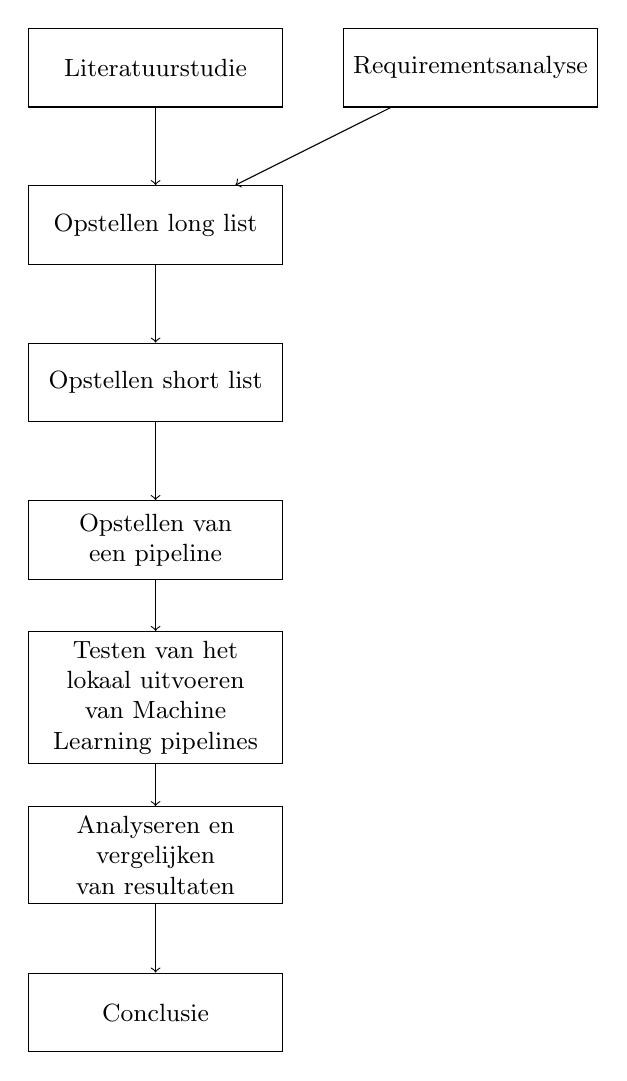
\begin{tikzpicture}[node distance=2cm, every node/.style={font=\small}]
  \node (pro0) [rectangle, draw, minimum width=3cm, minimum height=1cm, text centered, text width=3cm] {Literatuurstudie};
  \node (pro8) [rectangle, draw, minimum width=3cm, minimum height=1cm, text centered, text width=3cm, right of=pro0, xshift=2cm] {Requirements\-analyse};
  \node (pro1) [rectangle, draw, minimum width=3cm, minimum height=1cm, text centered, text width=3cm,below of=pro0] {Opstellen long list};
  \node (pro3) [rectangle, draw, minimum width=3cm, minimum height=1cm, text centered, text width=3cm, below of=pro1] {Opstellen short list};
  \node (pro4) [rectangle, draw, minimum width=3cm, minimum height=1cm, text centered, text width=3cm, below of=pro3] {Opstellen van een pipeline};
  \node (pro5) [rectangle, draw, minimum width=3cm, minimum height=1cm, text centered, text width=3cm, below of=pro4] {Testen van het lokaal uitvoeren van Machine Learning pipelines};
  \node (pro6) [rectangle, draw, minimum width=3cm, minimum height=1cm, text centered, text width=3cm, below of=pro5] {Analyseren en vergelijken van resultaten};
  \node (pro7) [rectangle, draw, minimum width=3cm, minimum height=1cm, text centered, text width=3cm, below of=pro6] {Conclusie};

  \draw [->] (pro0) -- (pro1);
  \draw [->] (pro1) -- (pro3);
  \draw [->] (pro3) -- (pro4);
  \draw [->] (pro4) -- (pro5);
  \draw [->] (pro5) -- (pro6);
  \draw [->] (pro6) -- (pro7);
  \draw [->] (pro8) -- (pro1);
\end{tikzpicture}

%% TODO: In dit hoofstuk geef je een korte toelichting over hoe je te werk bent
%% gegaan. Verdeel je onderzoek in grote fasen, en licht in elke fase toe wat
%% de doelstelling was, welke deliverables daar uit gekomen zijn, en welke
%% onderzoeksmethoden je daarbij toegepast hebt. Verantwoord waarom je
%% op deze manier te werk gegaan bent.
%% 
%% Voorbeelden van zulke fasen zijn: literatuurstudie, opstellen van een
%% requirements-analyse, opstellen long-list (bij vergelijkende studie),
%% selectie van geschikte tools (bij vergelijkende studie, "short-list"),
%% opzetten testopstelling/PoC, uitvoeren testen en verzamelen
%% van resultaten, analyse van resultaten, ...
%%
%% !!!!! LET OP !!!!!
%%
%% Het is uitdrukkelijk NIET de bedoeling dat je het grootste deel van de corpus
%% van je bachelorproef in dit hoofstuk verwerkt! Dit hoofdstuk is eerder een
%% kort overzicht van je plan van aanpak.
%%
%% Maak voor elke fase (behalve het literatuuronderzoek) een NIEUW HOOFDSTUK aan
%% en geef het een gepaste titel.



% Voeg hier je eigen hoofdstukken toe die de ``corpus'' van je bachelorproef
% vormen. De structuur en titels hangen af van je eigen onderzoek. Je kan bv.
% elke fase in je onderzoek in een apart hoofdstuk bespreken.

%\input{...}
%\input{...}
%...

%%=============================================================================
%% Conclusie
%%=============================================================================

\chapter{Conclusie}%
\label{ch:conclusie}

% TODO: Trek een duidelijke conclusie, in de vorm van een antwoord op de
% onderzoeksvra(a)g(en). Wat was jouw bijdrage aan het onderzoeksdomein en
% hoe biedt dit meerwaarde aan het vakgebied/doelgroep? 
% Reflecteer kritisch over het resultaat. In Engelse teksten wordt deze sectie
% ``Discussion'' genoemd. Had je deze uitkomst verwacht? Zijn er zaken die nog
% niet duidelijk zijn?
% Heeft het onderzoek geleid tot nieuwe vragen die uitnodigen tot verder 
%onderzoek?


% TODO: zorg ervoor dat je alle onderzoeksvragen beantwoord
% TODO: zorg voor een minder lange tekst, verdeel hem in meerdere paragrafen

Het probleem dat zich voordoet bij de huidige uitvoering van Machine Learning pipelines is dat deze bijna altijd in de cloud worden uitgevoerd. De cloud biedt veel opties en tarieven, waardoor dit voor studenten niet haalbaar is vanwege de kosten.
Daarom is in dit onderzoek gekeken naar de mogelijkheid om Machine Learning pipelines lokaal uit te voeren om dit probleem aan te pakken. Verschillende frameworks die lokaal Machine Learning pipelines kunnen uitvoeren, worden vergeleken. De voor- en nadelen van elk framework worden geanalyseerd, zodat het beste framework kan worden gekozen.
Na het analyseren van deze frameworks is de keuze gevallen op het Prefect framework. Prefect heeft een gebruiksvriendelijke interface, is schaalbaar met de cloud en biedt veel functies voor het beheren en ontwikkelen van Machine Learning pipelines. Dit framework zorgt er ook voor dat de code in dezelfde structuur als een normale Machine Learning pipeline kan blijven, in vergelijking met andere frameworks waarbij de code nog moet worden aangepast op basis van het doel van het project.
Alle frameworks zijn in staat om een Machine Learning Pipeline uit te voeren, maar velen zijn beperkt tot tekstgebaseerde Machine Learning pipelines. Dit onderzoek maakte gebruik van een image classification en alleen Prefect kon dit zonder veel aanpassingen uitvoeren als een Machine Learning pipeline. De andere frameworks hadden problemen met het doorgeven van variabelen, waardoor het langer duurde om een normale Machine Learning pipeline over te zetten naar het gekozen framework.
Prefect biedt ook meer functionaliteiten dan andere frameworks, zoals monitoring, herstarten van mislukte flows, plannen van uitvoeringen en een goed overzicht van alle flows. Het gebruik van Prefect biedt een goede basis voor het lokaal uitvoeren van Machine Learning pipelines.
Hierdoor kan Prefect worden beschouwd als een waardevol instrument voor data scientists en data engineers die op zoek zijn naar een betrouwbare oplossing voor het beheren van hun Machine Learning-workflows in een lokale omgeving.




%---------- Bijlagen -----------------------------------------------------------

\appendix

\chapter{Onderzoeksvoorstel}

Het onderwerp van deze bachelorproef is gebaseerd op een onderzoeksvoorstel dat vooraf werd beoordeeld door de promotor. Dat voorstel is opgenomen in deze bijlage.

%% TODO: 
%\section*{Samenvatting}

% Kopieer en plak hier de samenvatting (abstract) van je onderzoeksvoorstel.

% Verwijzing naar het bestand met de inhoud van het onderzoeksvoorstel
%---------- Inleiding ---------------------------------------------------------

\section{Introductie}%
\label{sec:introductie}

De toename van Artificiële Intelligentie (AI), Machine Learning (ML) en Deep Learning heeft geleid tot een groeiende vraag naar manieren om Machine Learning modellen op een schaalbare en efficiënte manier te implementeren en te beheren \autocite{Aggarwal2022}.
Binnen het keuzepakket ``AI \& Data Engineering'' right het opleidingsonderdeel ``Machine Learning Operations'' zich op het opzetten van machine learning werkruimtes en het monitoren van machine learning operaties. In dit vak leert de student complexe IT-oplossingen efficiënt en zelfstandig te installeren, configureren, beveiligen, onderhouden en aanpassen, zodat ze blijven voldoen aan de veranderende behoeften. De student leert ook de CI/CD-principes toe te passen binnen de context van machine learning, zoals het beschrijven van deze principes, het in productie brengen en monitoren van een machine learning model met behulp van CI/CD-principes. Verder kan de student de uitdagingen en mogelijke oplossingen beschrijven voor het draaien van een machine learning model op apparaten met beperkte rekenkracht, en het model laten werken op zo'n apparaat, bijvoorbeeld door gebruik te maken van TensorFlow Lite.
Dit onderzoek richt zich op een specifieke uitdaging binnen Machine Learning Operations: het lokaal uitvoeren van Machine Learning pipelines.

In het kader van dit opleidingsonderdeel wordt er gebruik gemaakt van Azure ML pipelines, waarvan het onderliggende framework Kubeflow is. Kubeflow is een open-source Machine Learning toolkit op Kubernetes \autocite{Kubeflow2021}.
Het gebruik van Azure ML pipelines is namelijk niet gratis voor studenten die niet genoeg krediet hebben op het platform. Dit leidt ertoe dat dit onderzoek zich richt op het lokaal uitvoeren van machine learning pipelines.
Het lokaal uitvoeren van Machine Learning pipelines kan ook problemen met zich meebrengen, zoals de noodzaak van veel rekenkracht die mogelijk niet beschikbaar is op computers van studenten. Als gevolg daarvan hebben bepaalde frameworks een beperkte versie die niet zo krachtig is als de cloud-variant, maar toch lokaal Machine Learning pipelines kan uitvoeren.
Er zal onderzoek gedaan worden naar alternatieve frameworks om Machine Learning pipelines lokaal uit te voeren. Deze zullen met elkaar worden vergeleken om vervolgens een Proof of Concept (PoC) op te stellen. Hierbij zal gekeken worden naar hoe de verschillende frameworks en bibliotheken werken, welke programmeertaal ze gebruiken en welke functies ze aanbieden. Daarnaast worden de frameworks getest op de compatibiliteit met verschillende besturingssystemen. Deze test omvat gedetailleerde installaties van alle frameworks, waarvan de resultaten worden vastgelegd in een rapport.

Dit onderzoek richt zich op IT-professionals die betrokken zijn bij Machine Learning Operations, specifiek voor de diegenen die ML-pipelines lokaal willen uitvoeren.
Het lokaal uitvoeren van Machine Learning pipelines blijkt een uitdaging te zijn, vooral met betrekking tot de huidige migratieproblemen en gebrekkige documentatie.
De centrale onderzoeksvraag is daarom: ``Hoe kan een ML-pipeline lokaal worden uitgevoerd met behulp van een Machine Learning framework?''
Hierbij worden de volgende deelvragen behandeld:
\begin{itemize}
  \item Wat zijn de belangrijkste uitdagingen bij het lokaliseren van Machine Learning pipelines?
  \item Welke specifieke problemen kunnen optreden bij het lokaal uitvoeren van Machine\\ Learning pipelines?
  \item Hoe vertaalt de lokale uitvoering van een ML pipeline zich naar de cloud?
  \item Wat zijn de hardware- en softwarevereisten voor het lokaal uitvoeren van een ML-pipeline?
  \item Welke frameworks en tools kunnen worden gebruikt om Machine Learning pipelines lokaal uit te voeren, en wat zijn hun respectieve kenmerken en voordelen?
\end{itemize}


%---------- Stand van zaken ---------------------------------------------------

\section{Literatuurstudie}%
\label{sec:state-of-the-art}

De exponentiële groei van Machine Learning heeft niet alleen het onderzoeksdomein beïnvloed, maar heeft de implementatie van Machine Learning pipelines tot leven gebracht \autocite{Aggarwal2022}.
Deze literatuurstudie werpt een diepgaande blik op het lokaal uitvoeren van Machine Learning pipelines.
De focus van deze literatuurstudie zal liggen op de fundamentele elementen van Machine Learning pipelines, zoals de definitie van Machine Learning en pipelines, evenals een overzicht van de beschikbare frameworks voor het lokale uitvoeren van Machine Learning pipelines.
\subsection{Machine Learning}
Machine Learning (ML) is een onderliggend deel van Artificiële Intelligentie (AI), een snel groeiend vakgebied op het raakvlak van data en statistiek dat feitgebaseerde beslissingen in verschillende sectoren aanstuurt \autocite{Jordan2015}.
Middels het toepassen van wiskundige principes kan Machine Learning verbanden leggen tussen gegevens om betrouwbare voorspellingen te genereren. Dit wordt mogelijk gemaakt door het gebruik van Machine Learning algoritmen, waarmee computers kunnen leren van data. Met gebruik van iteratieve testen en validatie kunnen ze hun prestaties in de loop van de tijd verbeteren, waardoor ze nieuwe taken kunnen uitvoeren met nieuwe data \autocite{Shaveta2023}.
\subsection{CI/CD pipelines}
Een Continuous Integration/Continuous Deployment (CI/CD) pipeline vormt een cruciaal onderdeel van moderne softwareontwikkeling, gericht op het versnellen en betrouwbaarder maken van de levering van webapplicaties \autocite{Singh2023}. Deployment binnen de pipeline verwijst naar het proces van het implementeren van nieuwe code of updates naar de productieomgeving, terwijl delivery verwijst naar het proces van het gereed maken van nieuwe code of updates voor implementatie. De effectiviteit van deze pipelines is sterk afhankelijk van regelmatig onderhoud en updates om gelijke tred te houden met veranderingen in systemen en technologieën. Binnen het domein van datamanagement benadrukken \textcite{Samad2018} en \textcite{Vadavalasa2020} respectievelijk de cruciale aspecten van het optimaliseren van beperkte datasets en de implementatie van Continuous Integration in de datapipeline. Deze inzichten vormen de kern van een intrigerend verhaal dat draait om de zoektocht naar efficiëntie en effectiviteit bij het omgaan met gegevens. In deze studies wordt ook aangetoond dat het verzamelen van data veel geld kan kosten en veel tijd in beslag kan nemen. Verder tonen deze studies aan dat nauwkeurige modellen kunnen worden gegenereerd met behulp van ML-pipelines en een beperkte dataset. Dit onderzoeksvoorstel benadrukt ook de bijdragen van \textcite{Zhang2022} als belangrijke figuren met hun eigen inzichten.
\textcite{Zhang2022} richten zich op het ontwerpen en automatiseren van datapipelines. Hij toont aan dat met behulp van datapipelines dat een Machine Learning model veel efficiënter kan worden getraind, omdat de data goed wordt schoongemaakt en verwerkt, zodat onnodige of ontbrekende data niet de accuraatheid van het model beïnvloedt.
\subsection{Machine Learning frameworks en libraries}
De ontwikkeling van Machine Learning (ML) frameworks en bibliotheken heeft in de afgelopen 25 jaar een aanzienlijke vooruitgang gekend \autocite{Nguyen2019}. Deze tools hebben als gemeenschappelijk doel om de complexe\newline data-analyseprocessen te vergemakkelijken en geïntegreerde omgevingen te bieden bovenop standaard programmeertalen. Ze zijn ontworpen voor diverse doeleinden, variërend van analytische platformen, voorspellende systemen tot aanbevelingssystemen en verwerkingstools voor beeld-, geluids- of taaldata. Sommige zijn gericht op snelle verwerking en streaming van grootschalige data, terwijl andere gespecialiseerd zijn in het implementeren van ML-algoritmen, waaronder Neurale Netwerken (NNs) en Deep Learning (DL). Het is belangrijk om te benadrukken dat er geen enkele tool is die geschikt is voor elk probleem, en vaak is een combinatie van tools nodig om succesvol te zijn.

\subsubsection{Kubeflow}
\textcite{Kubeflow2021} is een open-source platform dat een collectie van Machine Learning tools biedt die compatibel zijn met Kubernetes. Het wordt vooral gebruikt in DevOps-frameworks, waar het Machine Learning stacks en componenten zoals PyTorch en TensorFlow kan beheren \autocite{Chandana2021}.

Kubeflow kan ook gebruikt worden bij end-to-end Machine Learning oplossingen, waarbij pipelineonderdelen de uitvoering van taken en het beheer van artefacten vereenvoudigen \autocite{Bisong2019}.

Met Kubeflow kunnen teams profiteren van herbruikbare ML-componenten, zoals TensorFlow en PyTorch, terwijl ze tegelijkertijd gebruikmaken van Kubernetes voorzieningen voor schaalbaarheid, betrouwbaarheid en flexibiliteit. De samenwerking tussen Kubernetes en Kubeflow stelt organisaties in staat om Machine Learning processen te versnellen en te vereenvoudigen, waardoor ze snel kunnen reageren op de eisen van een dynamische markt.

\subsubsection{Kedro}
\textcite{Kedro2024} biedt een gestructureerde aanpak voor het bouwen van datapipelines door gebruik te maken van best practices en industriestandaarden. Met Kedro kunnen data engineers op een collaboratieve en efficiënte manier werken aan projecten, vanaf de initiële toestroom van data tot aan de implementatie van geavanceerde Machine Learning modellen.
De kracht van Kedro ligt in zijn flexibiliteit en modulariteit. Het framework heeft een componentgebaseerde architectuur, waardoor gebruikers herbruikbare en onderhoudbare code kunnen creëren. Kedro maakt het mogelijk om op een gestructureerde manier te werken aan complexe datapipelines, waardoor de ontwikkelingstijd wordt verkort en de betrouwbaarheid van datapipelines wordt verbeterd.
\subsubsection{MLflow}
MLflow benadrukt gebruiksgemak en aanpasbaarheid. Het biedt een gestandaardiseerde manier om machine learning projecten te beheren, ongeacht de programmeertaal die wordt gebruikt. Met MLflow kunnen experimenten worden bijgehouden, modelparameters worden geregistreerd, modellen worden beheerd en zelfs modellen worden geïmplementeerd in verschillende omgevingen.
De belangrijkste pijlers van MLflow zijn Tracking, Projects, Models en Registry. Tracking biedt een eenvoudige manier om experimenten te volgen en resultaten te vergelijken. Projects zorgen voor een uniforme structuur voor machine learning projecten en bevorderen de herbruikbaarheid. Models biedt tools om modellen in te pakken en te implementeren in verschillende omgevingen, terwijl Registry fungeert als een centrale hub voor het beheren van modelversies.

%Hier beschrijf je de \emph{state-of-the-art} rondom je gekozen onderzoeksdomein, d.w.z.\ een inleidende, doorlopende tekst over het onderzoeksdomein van je bachelorproef. Je steunt daarbij heel sterk op de professionele \emph{vakliteratuur}, en niet zozeer op populariserende teksten voor een breed publiek. Wat is de huidige stand van zaken in dit domein, en wat zijn nog eventuele open vragen (die misschien de aanleiding waren tot je onderzoeksvraag!)?

%Je mag de titel van deze sectie ook aanpassen (literatuurstudie, stand van zaken, enz.). Zijn er al gelijkaardige onderzoeken gevoerd? Wat concluderen ze? Wat is het verschil met jouw onderzoek?

%Verwijs bij elke introductie van een term of bewering over het domein naar de vakliteratuur, bijvoorbeeld~\autocite{Hykes2013}! Denk zeker goed na welke werken je refereert en waarom.

%Draag zorg voor correcte literatuurverwijzingen! Een bronvermelding hoort thuis \emph{binnen} de zin waar je je op die bron baseert, dus niet er buiten! Maak meteen een verwijzing als je gebruik maakt van een bron. Doe dit dus \emph{niet} aan het einde van een lange paragraaf. Baseer nooit teveel aansluitende tekst op eenzelfde bron.

%Als je informatie over bronnen verzamelt in JabRef, zorg er dan voor dat alle nodige info aanwezig is om de bron terug te vinden (zoals uitvoerig besproken in de lessen Research Methods).

% Voor literatuurverwijzingen zijn er twee belangrijke commando's:
% \autocite{KEY} => (Auteur, jaartal) Gebruik dit als de naam van de auteur
%   geen onderdeel is van de zin.
% \textcite{KEY} => Auteur (jaartal)  Gebruik dit als de auteursnaam wel een
%   functie heeft in de zin (bv. ``Uit onderzoek door Doll & Hill (1954) bleek
%   ...'')

%Je mag deze sectie nog verder onderverdelen in subsecties als dit de structuur van de tekst kan verduidelijken.

%---------- Methodologie ------------------------------------------------------
\section{Methodologie}%
\label{sec:methodologie}
Het onderzoek is onderverdeeld in verschillende fasen om een grondige evaluatie uit te voeren van de mogelijkheden en prestaties van verschillende frameworks en bibliotheken die Machine Learning pipelines ondersteunen. Elke fase heeft een specifieke focus en draagt bij aan het uiteindelijke doel van het ontwikkelen van een effectieve methode voor het lokaal uitvoeren van Machine Learning pipelines.
\subsection{Fase 1: Literatuurstudie (2 weken)}
Er zal een literatuurstudie worden uitgevoerd om inzicht te krijgen in de werking en
functies van verschillende frameworks en bibliotheken die Machine Learning pipelines ondersteunen.
Deze literatuurstudie zal gericht zijn op het vaststellen van mogelijke manieren om Machine Learning pipelines lokaal te uitvoeren. Er zal ook gekeken worden naar de gelijkenissen en verschillen van de frameworks en de compatibiliteit met verschillende besturingssystemen zoals Windows, Linux en macOS.
Als resultaat zal een samenvatting geschreven worden met alle relevante informatie voor dit onderzoek.
\subsection{Fase 2: Requirementsanalyse (2 weken)}
In de requirementanalyse fase worden de vereisten voor de lokale ML pipeline opgesteld, in samenwerking met de copromotor. Deze vereisten omvatten alle functionele en niet-functionele vereisten die nodig zijn voor het ontwikkelen van de Proof of Concept.

\subsection{Fase 3: Long list (2 weken)}
Binnen deze fase wordt een long list samengesteld van mogelijke frameworks die potentieel bruikbaar kunnen zijn. Een methodologie gericht op grondig online onderzoek, evenals het doorzoeken van verschillende frameworks en bibliotheken wordt toegepast om een uitgebreide lijst van bronnen te verzamelen. Deze bronnen zijn geselecteerd vanwege hun potentie om waardevolle informatie te bieden die relevant is voor het vergelijken van de frameworks.
\subsection{Fase 4: Short list (1 week)}
Met behulp van de long list zullen we elke oplossing grondig analyseren en beoordelen aan de hand van de vereisten die zijn vastgesteld in de requirementsanalyse. Dit zal bepalen welke vereisten zijn vervuld, welke niet zijn vervuld en welke mogelijk onduidelijk zijn. Het uiteindelijke resultaat van deze fase zal één of twee mogelijke benaderingen zijn voor het ontwikkelen van het Proof of Concept.
\subsection{Fase 5: Het maken van een ML-pipeline (2 weken)}
In deze fase wordt een reeks pipelines ontwikkeld om de verschillende frameworks te testen die lokaal Machine Learning pipelines uitvoeren. Deze pipelines worden ontworpen om het gedrag en de prestaties van de frameworks grondig te evalueren en te vergelijken. Elke pipeline zal gebruikmaken van dezelfde dataset en algoritmes om Machine Learning modellen te genereren. Dit proces stelt ons in staat om nauwkeurige beoordelingen te maken van de mogelijkheden en beperkingen van de verschillende frameworks en om weloverwogen beslissingen te nemen bij de keuze van het meest geschikte framework voor het beoogde doel.
\subsection{Fase 6: Proof of Concept (4 weken)}
De Proof of Concept zal bestaan uit testen die worden uitgevoerd op de gekozen frameworks. Eerst zal de installatie worden uitgevoerd en zal elke stap beschreven en geanalyseerd worden om in kaart te brengen of er fouten voorkomen. Vervolgens wordt onderzocht hoe de frameworks lokaal worden opgezet en gebruikt. Hiervoor zal er een pipeline gemaakt worden die altijd dezelfde data verwerkt en bewerkingen uitvoert. Dit resultaat zal worden bijgehouden in een rapport.
Deze testen zullen op verschillende besturingssystemen worden uitgevoerdn zoals Windows, Linux en macOS, en met verschillende soorten data. Hierdoor zal dit onderzoek over meer data beschikken en zullen de uiteindelijke conclusies beter onderbouwd kunnen worden.

Na het verzamelen van de nodige data van de verschillende testen wordt dit ook verder geanalyseerd. Hierbij worden de resultaten van de verschillende testen vergeleken aan de hand van verschillende criteria, waaronder:
\begin{itemize}
  \item \textbf{Installatieproces en -tijd:} De soepelheid en snelheid van de installatie op verschillende besturingssystemen worden geanalyseerd.
  \item \textbf{Uitvoering van de pipeline:} Er wordt onderzocht hoe de pipelines worden uitgevoerd op de verschillende frameworks en bibliotheken, met speciale aandacht voor consistentie en snelheid van uitvoering.
  \item \textbf{Tijd voor het uitvoeren van pipelines:} De tijd die nodig is om de pipelines uit te voeren op de verschillende frameworks en bibliotheken wordt vergeleken om prestatieverschillen te identificeren.
  \item \textbf{Voldoen aan vereisten:} Elk framework of bibliotheek wordt geëvalueerd op de mate waarin het voldoet aan de eerder geïdentificeerde requirements.
  \item \textbf{Stabiliteit en betrouwbaarheid:} De stabiliteit en betrouwbaarheid van de frameworks en bibliotheken worden beoordeeld aan de hand van eventuele fouten of crashes tijdens de testen.
\end{itemize}
Op deze manier wordt er gekeken hoe effectief de verschillende frameworks en bibliotheken de Machine Learning pipelines lokaal kunnen uitvoeren. Tot slot wordt op basis van de geanalyseerde data een conclusie geformuleerd.\\
\subsection{Fase 7: Conclusie (2 weken)}
Het uiteindelijke resultaat van dit onderzoek zal een volledig rapport zijn waarin de bevindingen en conclusies gedetailleerd beschreven worden alsook een oplossing voor het lokaal uitvoeren van Machine Learning pipelines. Dit zal stapsgewijs gebeuren, waarin de belangrijkste bevindingen en conclusies worden aangetoond.\\

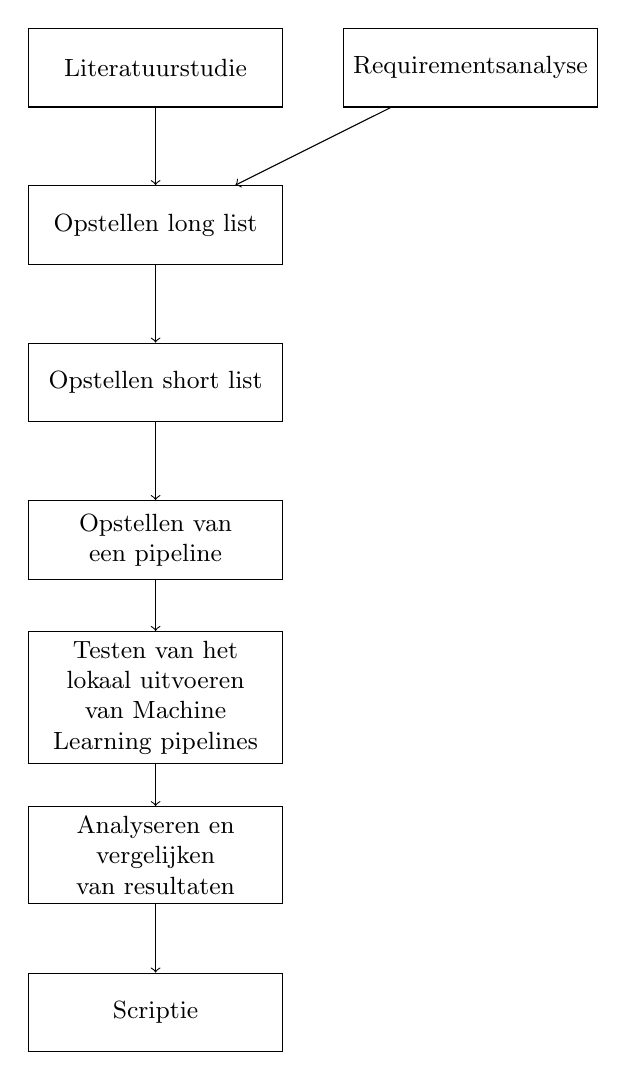
\begin{tikzpicture}[node distance=2cm, every node/.style={font=\small}]
  \node (pro0) [rectangle, draw, minimum width=3cm, minimum height=1cm, text centered, text width=3cm] {Literatuurstudie};
  \node (pro8) [rectangle, draw, minimum width=3cm, minimum height=1cm, text centered, text width=3cm, right of=pro0, xshift=2cm] {Requirements\-analyse};
  \node (pro1) [rectangle, draw, minimum width=3cm, minimum height=1cm, text centered, text width=3cm,below of=pro0] {Opstellen long list};
  \node (pro3) [rectangle, draw, minimum width=3cm, minimum height=1cm, text centered, text width=3cm, below of=pro1] {Opstellen short list};
  \node (pro4) [rectangle, draw, minimum width=3cm, minimum height=1cm, text centered, text width=3cm, below of=pro3] {Opstellen van een pipeline};
  \node (pro5) [rectangle, draw, minimum width=3cm, minimum height=1cm, text centered, text width=3cm, below of=pro4] {Testen van het lokaal uitvoeren van Machine Learning pipelines};
  \node (pro6) [rectangle, draw, minimum width=3cm, minimum height=1cm, text centered, text width=3cm, below of=pro5] {Analyseren en vergelijken van resultaten};
  \node (pro7) [rectangle, draw, minimum width=3cm, minimum height=1cm, text centered, text width=3cm, below of=pro6] {Scriptie};

  \draw [->] (pro0) -- (pro1);
  \draw [->] (pro1) -- (pro3);
  \draw [->] (pro3) -- (pro4);
  \draw [->] (pro4) -- (pro5);
  \draw [->] (pro5) -- (pro6);
  \draw [->] (pro6) -- (pro7);
  \draw [->] (pro8) -- (pro1);
\end{tikzpicture}


%Hier beschrijf je hoe je van plan bent het onderzoek te voeren. Welke onderzoekstechniek ga je toepassen om elk van je onderzoeksvragen te beantwoorden? Gebruik je hiervoor literatuurstudie, interviews met belanghebbenden (bv.~voor requirements-analyse), experimenten, simulaties, vergelijkende studie, risico-analyse, PoC, \ldots?

%Valt je onderwerp onder één van de typische soorten bachelorproeven die besproken zijn in de lessen Research Methods (bv.\ vergelijkende studie of risico-analyse)? Zorg er dan ook voor dat we duidelijk de verschillende stappen terug vinden die we verwachten in dit soort onderzoek!

%Vermijd onderzoekstechnieken die geen objectieve, meetbare resultaten kunnen opleveren. Enquêtes, bijvoorbeeld, zijn voor een bachelorproef informatica meestal \textbf{niet geschikt}. De antwoorden zijn eerder meningen dan feiten en in de praktijk blijkt het ook bijzonder moeilijk om voldoende respondenten te vinden. Studenten die een enquête willen voeren, hebben meestal ook geen goede definitie van de populatie, waardoor ook niet kan aangetoond worden dat eventuele resultaten representatief zijn.

%Uit dit onderdeel moet duidelijk naar voor komen dat je bachelorproef ook technisch voldoen\-de diepgang zal bevatten. Het zou niet kloppen als een bachelorproef informatica ook door bv.\ een student marketing zou kunnen uitgevoerd worden.

%Je beschrijft ook al welke tools (hardware, software, diensten, \ldots) je denkt hiervoor te gebruiken of te ontwikkelen.

%Probeer ook een tijdschatting te maken. Hoe lang zal je met elke fase van je onderzoek bezig zijn en wat zijn de concrete \emph{deliverables} in elke fase?

%---------- Verwachte resultaten ----------------------------------------------
\section{Verwacht resultaat, conclusie}%
\label{sec:verwachte_resultaten}
Dit onderzoek heeft als doel om personen in het vakgebied Machine Learning Operations te voorzien van een duidelijke aanbeveling voor het lokaal uitvoeren van Machine Learning pipelines. Het verwachte resultaat omvat een overzicht van beschikbare frameworks en bibliotheken, met de identificatie van de meest veelbelovende opties op basis van criteria zoals installatiegemak, prestaties en compatibiliteit. Het onderzoek zal praktische testresultaten presenteren die laten zien hoe deze geselecteerde tools presteren in de praktijk. Een conclusie en aanbeveling zullen worden geformuleerd op basis van deze resultaten, samen met beknopte praktische richtlijnen voor het gebruik van het aanbevolen framework of bibliotheek. Bovendien zal het onderzoek inzicht verschaffen in de uitdagingen en mogelijke obstakels bij het lokaal uitvoeren van Machine Learning pipelines.

%Hier beschrijf je welke resultaten je verwacht. Als je metingen en simulaties uitvoert, kan je hier al mock-ups maken van de grafieken samen met de verwachte conclusies. Benoem zeker al je assen en de onderdelen van de grafiek die je gaat gebruiken. Dit zorgt ervoor dat je concreet weet welk soort data je moet verzamelen en hoe je die moet meten.

%Wat heeft de doelgroep van je onderzoek aan het resultaat? Op welke manier zorgt jouw bachelorproef voor een meerwaarde?

%Hier beschrijf je wat je verwacht uit je onderzoek, met de motivatie waarom. Het is \textbf{niet} erg indien uit je onderzoek andere resultaten en conclusies vloeien dan dat je hier beschrijft: het is dan juist interessant om te onderzoeken waarom jouw hypothesen niet overeenkomen met de resultaten.

%%---------- Andere bijlagen --------------------------------------------------
% TODO: Voeg hier eventuele andere bijlagen toe. Bv. als je deze BP voor de
% tweede keer indient, een overzicht van de verbeteringen t.o.v. het origineel.
%\input{...}

%%---------- Backmatter, referentielijst ---------------------------------------

\backmatter{}

\setlength\bibitemsep{2pt} %% Add Some space between the bibliograpy entries
\printbibliography[heading=bibintoc]

\end{document}
